% Generated by Sphinx.
\def\sphinxdocclass{report}
\documentclass[letterpaper,10pt,english]{sphinxmanual}
\usepackage[utf8]{inputenc}
\DeclareUnicodeCharacter{00A0}{\nobreakspace}
\usepackage{cmap}
\usepackage[T1]{fontenc}
\usepackage{babel}
\usepackage{times}
\usepackage[Bjarne]{fncychap}
\usepackage{longtable}
\usepackage{sphinx}
\usepackage{multirow}


\title{Méthodes numériques Documentation}
\date{December 18, 2014}
\release{0.0.1}
\author{ENSAM}
\newcommand{\sphinxlogo}{}
\renewcommand{\releasename}{Release}
\makeindex

\makeatletter
\def\PYG@reset{\let\PYG@it=\relax \let\PYG@bf=\relax%
    \let\PYG@ul=\relax \let\PYG@tc=\relax%
    \let\PYG@bc=\relax \let\PYG@ff=\relax}
\def\PYG@tok#1{\csname PYG@tok@#1\endcsname}
\def\PYG@toks#1+{\ifx\relax#1\empty\else%
    \PYG@tok{#1}\expandafter\PYG@toks\fi}
\def\PYG@do#1{\PYG@bc{\PYG@tc{\PYG@ul{%
    \PYG@it{\PYG@bf{\PYG@ff{#1}}}}}}}
\def\PYG#1#2{\PYG@reset\PYG@toks#1+\relax+\PYG@do{#2}}

\expandafter\def\csname PYG@tok@gd\endcsname{\def\PYG@tc##1{\textcolor[rgb]{0.63,0.00,0.00}{##1}}}
\expandafter\def\csname PYG@tok@gu\endcsname{\let\PYG@bf=\textbf\def\PYG@tc##1{\textcolor[rgb]{0.50,0.00,0.50}{##1}}}
\expandafter\def\csname PYG@tok@gt\endcsname{\def\PYG@tc##1{\textcolor[rgb]{0.00,0.27,0.87}{##1}}}
\expandafter\def\csname PYG@tok@gs\endcsname{\let\PYG@bf=\textbf}
\expandafter\def\csname PYG@tok@gr\endcsname{\def\PYG@tc##1{\textcolor[rgb]{1.00,0.00,0.00}{##1}}}
\expandafter\def\csname PYG@tok@cm\endcsname{\let\PYG@it=\textit\def\PYG@tc##1{\textcolor[rgb]{0.25,0.50,0.56}{##1}}}
\expandafter\def\csname PYG@tok@vg\endcsname{\def\PYG@tc##1{\textcolor[rgb]{0.73,0.38,0.84}{##1}}}
\expandafter\def\csname PYG@tok@m\endcsname{\def\PYG@tc##1{\textcolor[rgb]{0.13,0.50,0.31}{##1}}}
\expandafter\def\csname PYG@tok@mh\endcsname{\def\PYG@tc##1{\textcolor[rgb]{0.13,0.50,0.31}{##1}}}
\expandafter\def\csname PYG@tok@cs\endcsname{\def\PYG@tc##1{\textcolor[rgb]{0.25,0.50,0.56}{##1}}\def\PYG@bc##1{\setlength{\fboxsep}{0pt}\colorbox[rgb]{1.00,0.94,0.94}{\strut ##1}}}
\expandafter\def\csname PYG@tok@ge\endcsname{\let\PYG@it=\textit}
\expandafter\def\csname PYG@tok@vc\endcsname{\def\PYG@tc##1{\textcolor[rgb]{0.73,0.38,0.84}{##1}}}
\expandafter\def\csname PYG@tok@il\endcsname{\def\PYG@tc##1{\textcolor[rgb]{0.13,0.50,0.31}{##1}}}
\expandafter\def\csname PYG@tok@go\endcsname{\def\PYG@tc##1{\textcolor[rgb]{0.20,0.20,0.20}{##1}}}
\expandafter\def\csname PYG@tok@cp\endcsname{\def\PYG@tc##1{\textcolor[rgb]{0.00,0.44,0.13}{##1}}}
\expandafter\def\csname PYG@tok@gi\endcsname{\def\PYG@tc##1{\textcolor[rgb]{0.00,0.63,0.00}{##1}}}
\expandafter\def\csname PYG@tok@gh\endcsname{\let\PYG@bf=\textbf\def\PYG@tc##1{\textcolor[rgb]{0.00,0.00,0.50}{##1}}}
\expandafter\def\csname PYG@tok@ni\endcsname{\let\PYG@bf=\textbf\def\PYG@tc##1{\textcolor[rgb]{0.84,0.33,0.22}{##1}}}
\expandafter\def\csname PYG@tok@nl\endcsname{\let\PYG@bf=\textbf\def\PYG@tc##1{\textcolor[rgb]{0.00,0.13,0.44}{##1}}}
\expandafter\def\csname PYG@tok@nn\endcsname{\let\PYG@bf=\textbf\def\PYG@tc##1{\textcolor[rgb]{0.05,0.52,0.71}{##1}}}
\expandafter\def\csname PYG@tok@no\endcsname{\def\PYG@tc##1{\textcolor[rgb]{0.38,0.68,0.84}{##1}}}
\expandafter\def\csname PYG@tok@na\endcsname{\def\PYG@tc##1{\textcolor[rgb]{0.25,0.44,0.63}{##1}}}
\expandafter\def\csname PYG@tok@nb\endcsname{\def\PYG@tc##1{\textcolor[rgb]{0.00,0.44,0.13}{##1}}}
\expandafter\def\csname PYG@tok@nc\endcsname{\let\PYG@bf=\textbf\def\PYG@tc##1{\textcolor[rgb]{0.05,0.52,0.71}{##1}}}
\expandafter\def\csname PYG@tok@nd\endcsname{\let\PYG@bf=\textbf\def\PYG@tc##1{\textcolor[rgb]{0.33,0.33,0.33}{##1}}}
\expandafter\def\csname PYG@tok@ne\endcsname{\def\PYG@tc##1{\textcolor[rgb]{0.00,0.44,0.13}{##1}}}
\expandafter\def\csname PYG@tok@nf\endcsname{\def\PYG@tc##1{\textcolor[rgb]{0.02,0.16,0.49}{##1}}}
\expandafter\def\csname PYG@tok@si\endcsname{\let\PYG@it=\textit\def\PYG@tc##1{\textcolor[rgb]{0.44,0.63,0.82}{##1}}}
\expandafter\def\csname PYG@tok@s2\endcsname{\def\PYG@tc##1{\textcolor[rgb]{0.25,0.44,0.63}{##1}}}
\expandafter\def\csname PYG@tok@vi\endcsname{\def\PYG@tc##1{\textcolor[rgb]{0.73,0.38,0.84}{##1}}}
\expandafter\def\csname PYG@tok@nt\endcsname{\let\PYG@bf=\textbf\def\PYG@tc##1{\textcolor[rgb]{0.02,0.16,0.45}{##1}}}
\expandafter\def\csname PYG@tok@nv\endcsname{\def\PYG@tc##1{\textcolor[rgb]{0.73,0.38,0.84}{##1}}}
\expandafter\def\csname PYG@tok@s1\endcsname{\def\PYG@tc##1{\textcolor[rgb]{0.25,0.44,0.63}{##1}}}
\expandafter\def\csname PYG@tok@gp\endcsname{\let\PYG@bf=\textbf\def\PYG@tc##1{\textcolor[rgb]{0.78,0.36,0.04}{##1}}}
\expandafter\def\csname PYG@tok@sh\endcsname{\def\PYG@tc##1{\textcolor[rgb]{0.25,0.44,0.63}{##1}}}
\expandafter\def\csname PYG@tok@ow\endcsname{\let\PYG@bf=\textbf\def\PYG@tc##1{\textcolor[rgb]{0.00,0.44,0.13}{##1}}}
\expandafter\def\csname PYG@tok@sx\endcsname{\def\PYG@tc##1{\textcolor[rgb]{0.78,0.36,0.04}{##1}}}
\expandafter\def\csname PYG@tok@bp\endcsname{\def\PYG@tc##1{\textcolor[rgb]{0.00,0.44,0.13}{##1}}}
\expandafter\def\csname PYG@tok@c1\endcsname{\let\PYG@it=\textit\def\PYG@tc##1{\textcolor[rgb]{0.25,0.50,0.56}{##1}}}
\expandafter\def\csname PYG@tok@kc\endcsname{\let\PYG@bf=\textbf\def\PYG@tc##1{\textcolor[rgb]{0.00,0.44,0.13}{##1}}}
\expandafter\def\csname PYG@tok@c\endcsname{\let\PYG@it=\textit\def\PYG@tc##1{\textcolor[rgb]{0.25,0.50,0.56}{##1}}}
\expandafter\def\csname PYG@tok@mf\endcsname{\def\PYG@tc##1{\textcolor[rgb]{0.13,0.50,0.31}{##1}}}
\expandafter\def\csname PYG@tok@err\endcsname{\def\PYG@bc##1{\setlength{\fboxsep}{0pt}\fcolorbox[rgb]{1.00,0.00,0.00}{1,1,1}{\strut ##1}}}
\expandafter\def\csname PYG@tok@kd\endcsname{\let\PYG@bf=\textbf\def\PYG@tc##1{\textcolor[rgb]{0.00,0.44,0.13}{##1}}}
\expandafter\def\csname PYG@tok@ss\endcsname{\def\PYG@tc##1{\textcolor[rgb]{0.32,0.47,0.09}{##1}}}
\expandafter\def\csname PYG@tok@sr\endcsname{\def\PYG@tc##1{\textcolor[rgb]{0.14,0.33,0.53}{##1}}}
\expandafter\def\csname PYG@tok@mo\endcsname{\def\PYG@tc##1{\textcolor[rgb]{0.13,0.50,0.31}{##1}}}
\expandafter\def\csname PYG@tok@mi\endcsname{\def\PYG@tc##1{\textcolor[rgb]{0.13,0.50,0.31}{##1}}}
\expandafter\def\csname PYG@tok@kn\endcsname{\let\PYG@bf=\textbf\def\PYG@tc##1{\textcolor[rgb]{0.00,0.44,0.13}{##1}}}
\expandafter\def\csname PYG@tok@o\endcsname{\def\PYG@tc##1{\textcolor[rgb]{0.40,0.40,0.40}{##1}}}
\expandafter\def\csname PYG@tok@kr\endcsname{\let\PYG@bf=\textbf\def\PYG@tc##1{\textcolor[rgb]{0.00,0.44,0.13}{##1}}}
\expandafter\def\csname PYG@tok@s\endcsname{\def\PYG@tc##1{\textcolor[rgb]{0.25,0.44,0.63}{##1}}}
\expandafter\def\csname PYG@tok@kp\endcsname{\def\PYG@tc##1{\textcolor[rgb]{0.00,0.44,0.13}{##1}}}
\expandafter\def\csname PYG@tok@w\endcsname{\def\PYG@tc##1{\textcolor[rgb]{0.73,0.73,0.73}{##1}}}
\expandafter\def\csname PYG@tok@kt\endcsname{\def\PYG@tc##1{\textcolor[rgb]{0.56,0.13,0.00}{##1}}}
\expandafter\def\csname PYG@tok@sc\endcsname{\def\PYG@tc##1{\textcolor[rgb]{0.25,0.44,0.63}{##1}}}
\expandafter\def\csname PYG@tok@sb\endcsname{\def\PYG@tc##1{\textcolor[rgb]{0.25,0.44,0.63}{##1}}}
\expandafter\def\csname PYG@tok@k\endcsname{\let\PYG@bf=\textbf\def\PYG@tc##1{\textcolor[rgb]{0.00,0.44,0.13}{##1}}}
\expandafter\def\csname PYG@tok@se\endcsname{\let\PYG@bf=\textbf\def\PYG@tc##1{\textcolor[rgb]{0.25,0.44,0.63}{##1}}}
\expandafter\def\csname PYG@tok@sd\endcsname{\let\PYG@it=\textit\def\PYG@tc##1{\textcolor[rgb]{0.25,0.44,0.63}{##1}}}

\def\PYGZbs{\char`\\}
\def\PYGZus{\char`\_}
\def\PYGZob{\char`\{}
\def\PYGZcb{\char`\}}
\def\PYGZca{\char`\^}
\def\PYGZam{\char`\&}
\def\PYGZlt{\char`\<}
\def\PYGZgt{\char`\>}
\def\PYGZsh{\char`\#}
\def\PYGZpc{\char`\%}
\def\PYGZdl{\char`\$}
\def\PYGZhy{\char`\-}
\def\PYGZsq{\char`\'}
\def\PYGZdq{\char`\"}
\def\PYGZti{\char`\~}
% for compatibility with earlier versions
\def\PYGZat{@}
\def\PYGZlb{[}
\def\PYGZrb{]}
\makeatother

\begin{document}

\maketitle
\tableofcontents
\phantomsection\label{index::doc}


Contents:


\chapter{Simple introduction à Matlab}
\label{matlab::doc}\label{matlab:notes-cours-methodes-numeriques-s}\label{matlab:simple-introduction-a-matlab}\label{matlab:introduction-matlab}
introduction simple à matlab.


\chapter{Introduction aux méthodes numériques}
\label{introduction_methodes_numeriques:introduction-aux-methodes-numeriques}\label{introduction_methodes_numeriques::doc}\label{introduction_methodes_numeriques:introduction-methodes-numeriques}

\section{Exercice 1}
\label{introduction_methodes_numeriques:exercice1}\label{introduction_methodes_numeriques:exercice-1}\setbox0\vbox{
\begin{minipage}{0.95\linewidth}
\textbf{Objectif}

\medskip


Observer la différence entre le calcul \textbf{algébrique} et le calcul \textbf{numérique}
\end{minipage}}
\begin{center}\setlength{\fboxsep}{5pt}\shadowbox{\box0}\end{center}

1- Calculer \textbf{algébriquement} les expressions suivantes:
\begin{gather}
\begin{split}\begin{eqnarray}
x&=&0.6+0.2+0.2+0.2\\
y&=&\sqrt{2}*\sqrt{2}-2\\
z&=&1-3*(\dfrac{4}{3}-1)
\end{eqnarray}\end{split}\notag
\end{gather}

\bigskip\hrule{}\bigskip


2- Calculer \textbf{numériquement} les expressions ci-dessus en utilisant le logiciel \emph{Matlab} et le \textbf{format long} pour afficher les résultats

\begin{Verbatim}[commandchars=\\\{\}]
\PYG{c}{\PYGZpc{}mettre le format en long}
\PYG{n}{format} \PYG{n}{long}

\PYG{c}{\PYGZpc{}affectation de x avec un affichage}
\PYG{n}{x}\PYG{p}{=}\PYG{l+m+mf}{0.6}\PYG{o}{+}\PYG{l+m+mf}{0.2}\PYG{o}{+}\PYG{l+m+mf}{0.2}\PYG{o}{+}\PYG{l+m+mf}{0.2}

\PYG{c}{\PYGZpc{}calcul de y en utilisant la fonction racine(==\PYGZgt{} sqrt)}
\PYG{n}{y}\PYG{p}{=}\PYG{n+nb}{sqrt}\PYG{p}{(}\PYG{l+m+mi}{2}\PYG{p}{)}\PYG{o}{*}\PYG{n+nb}{sqrt}\PYG{p}{(}\PYG{l+m+mi}{2}\PYG{p}{)}\PYG{o}{\PYGZhy{}}\PYG{l+m+mi}{2}

\PYG{c}{\PYGZpc{}Calcul de la valeur de z}
\PYG{n}{z}\PYG{p}{=}\PYG{l+m+mi}{1}\PYG{o}{\PYGZhy{}}\PYG{l+m+mi}{3}\PYG{o}{*}\PYG{p}{(}\PYG{l+m+mf}{4.}\PYG{o}{/}\PYG{l+m+mi}{3}\PYG{o}{\PYGZhy{}}\PYG{l+m+mi}{1}\PYG{p}{)}
\end{Verbatim}

\begin{notice}{note}{Note:}\begin{itemize}
\item {} 
le \textbf{codage} en Matlab est en double précision, et la fonction \emph{format} ne change pas le codage mais plutôt l'affichage, pour les autres formats disponibles:

\begin{Verbatim}[commandchars=\\\{\}]
help format
\end{Verbatim}

\item {} 
dans le calcul de la formule de \textbf{z} on a utiliser \textbf{4./3} pour éviter la division entière.

\end{itemize}
\end{notice}


\section{Exercice 2}
\label{introduction_methodes_numeriques:exercice2}\label{introduction_methodes_numeriques:exercice-2}\setbox0\vbox{
\begin{minipage}{0.95\linewidth}
\textbf{Objectif}

\medskip


Comparer la représentation \textbf{tronquée} et la représentation \textbf{arrondie}.
\end{minipage}}
\begin{center}\setlength{\fboxsep}{5pt}\shadowbox{\box0}\end{center}

On considère le nombre réel \(x=\dfrac{1}{15}\)

1- Donner la représentation \textbf{tronquée} à 5 chiffres en base 10, l'erreur absolue et l'erreur relative.:

\begin{Verbatim}[commandchars=\\\{\}]
la valeur de x est:
x=0.0666666666...
\end{Verbatim}

donc la représentation tronquée est
\begin{gather}
\begin{split}\begin{eqnarray}
x_t&=&0.06666\\
E_{abs}&=&|x-x_t|=6.6\;10^{-6}\\
E_{rel}&=&\dfrac{|x-x_t|}{|x|}=1\;10^{-4}
\end{eqnarray}\end{split}\notag
\end{gather}

\bigskip\hrule{}\bigskip


2- Donner la représentation \textbf{arrondie} à 5 chiffres en base 10, avec l'erreur absolue et l'erreur relative.
\begin{gather}
\begin{split}\begin{eqnarray}
x_{arr}&=&0.06667\\
E_{abs}&=&|x-x_{arr}|=3.3\;10^{-6}\\
E_{rel}&=&\dfrac{|x-x_{arr}|}{|x|}=4\;10^{-5}
\end{eqnarray}\end{split}\notag
\end{gather}
3- Commenter les résultats.

\begin{notice}{note}{Note:}
l'erreur d'arrondie est inférieure à celle de troncature,
\end{notice}


\section{Exercice 3}
\label{introduction_methodes_numeriques:exercice3}\label{introduction_methodes_numeriques:exercice-3}\setbox0\vbox{
\begin{minipage}{0.95\linewidth}
\textbf{Objectif}

\medskip


Codage des nombres.
\end{minipage}}
\begin{center}\setlength{\fboxsep}{5pt}\shadowbox{\box0}\end{center}
\begin{enumerate}
\item {} 
Calculer la représentation du nombre \((101.11)_2\) dans la base 10.

\end{enumerate}

\textbf{partie entière}
\begin{gather}
\begin{split}(101)_2=\mathbf{1}*2^2+\mathbf{0}*2^{1}+\mathbf{1}*2^{0}=4+1=\mathbf{5}\end{split}\notag
\end{gather}
\textbf{partie réelle}
\begin{gather}
\begin{split}(.11)_2=\mathbf{1}*(\frac{1}{2})^1+\mathbf{1}*(\frac{1}{2})^2=\dfrac{1}{2}+\dfrac{1}{4}=0.75\end{split}\notag
\end{gather}
donc
\begin{gather}
\begin{split}\begin{equation}
(101.11)_2=5.75
\end{equation}\end{split}\notag
\end{gather}

\bigskip\hrule{}\bigskip

\begin{enumerate}
\setcounter{enumi}{1}
\item {} 
Calculer la représentation des nombres \(0.1\) et \(\dfrac{1}{3}\) dans la base \textbf{2}.

\end{enumerate}
\begin{gather}
\begin{split}\begin{array}[|l|c|r]
 \hline
  0.1*2=\mathbf{0}.2 & \rightarrow & rep=0.\mathbf{0} \\
  0.2*2=\mathbf{0}.4 & \rightarrow & rep=0.0\mathbf{0} \\
  0.4*2=\mathbf{0}.8 & \rightarrow & rep=0.00\mathbf{0} \\
  0.8*2=\mathbf{1}.6 & \rightarrow & rep=0.000\mathbf{1} \\
  0.6*2=\mathbf{1}.2 & \rightarrow & rep=0.0001\mathbf{1} \\
\end{array}\end{split}\notag
\end{gather}
La représentation de \(0.2\) est cyclique avec un cycle \(0011\)

donc
\begin{gather}
\begin{split}0.1=(0.0001100110011\ldots)\end{split}\notag
\end{gather}
de même pour \(\dfrac{1}{3}\) on trouve:

\begin{Verbatim}[commandchars=\\\{\}]
1/3=0.010101...
\end{Verbatim}


\bigskip\hrule{}\bigskip

\begin{enumerate}
\setcounter{enumi}{2}
\item {} 
Représenter dans la norme \emph{IEEE} les nombres:
\begin{enumerate}
\item {} 
x=-9.5

\item {} 
y=6.625

\item {} 
z= \(\frac{1}{10}\)

\end{enumerate}

\end{enumerate}

\textbf{Codage de y}

partie entière:

\begin{Verbatim}[commandchars=\\\{\}]
6=(4+2)=(110)\PYGZus{}2
\end{Verbatim}

partie réelle
\begin{gather}
\begin{split}\begin{array}[|l|c|r]
 \hline
  0.625*2=\mathbf{1}.25 & \rightarrow & 0.\mathbf{1} \\
  0.25*2=\mathbf{0}.5 & \rightarrow & 0.10 \\
  0.5*2=\mathbf{1} & \rightarrow & 0.101 \\
\end{array}\end{split}\notag
\end{gather}
donc:

\begin{Verbatim}[commandchars=\\\{\}]
\PYG{l+m+mf}{6.625}\PYG{o}{=}\PYG{l+m+mf}{110.101}
\end{Verbatim}

Mise en forme \textbf{normalisée} pour éliminer le bit fontôme:

\begin{Verbatim}[commandchars=\\\{\}]
\PYG{l+m+mf}{6.625}\PYG{o}{=}\PYG{l+m+mf}{1.10101}\PYG{o}{*}\PYG{l+m+mi}{2}\PYG{o}{\PYGZca{}}\PYG{l+m+mi}{2}
\end{Verbatim}

en \textbf{simple précision} on utilise \emph{8 bits} pour l'exposant donc la valeur du \textbf{décalage} est.
\begin{gather}
\begin{split}decalage=2^{(8-1)}-1=127\end{split}\notag
\end{gather}
donc l'exposant à coder est

\begin{Verbatim}[commandchars=\\\{\}]
\PYG{n}{E}\PYG{o}{=}\PYG{l+m+mi}{2}\PYG{o}{+}\PYG{l+m+mi}{127}\PYG{o}{=}\PYG{l+m+mi}{129}\PYG{o}{=}\PYG{p}{(}\PYG{l+m+mi}{10000001}\PYG{p}{)}
\end{Verbatim}

et la mantisse est la partie après la virgule, remplie de \(0\) \textbf{vers la droite} pour obtenir \emph{23 bits}:

\begin{Verbatim}[commandchars=\\\{\}]
\PYG{n}{M}\PYG{o}{=}\PYG{l+m+mi}{10101000000000000000000}
\end{Verbatim}

ce qui donne le codage de x.
\begin{gather}
\begin{split}x=\underbrace{1}_{signe}\;\underbrace{10000001}_{exposant}\;\underbrace{10101000000000000000000}_{mantisse}\end{split}\notag
\end{gather}
pour plus de détails voir (\href{http://fr.wikipedia.org/wiki/IEEE\_754}{IEEE\_754})


\bigskip\hrule{}\bigskip

\begin{enumerate}
\setcounter{enumi}{3}
\item {} 
Donner la représentation en simple précision sur un ordinateur du nombre \(+1101.1\)
\begin{itemize}
\item {} 
sans tenant compte du \textbf{bit fontôme}.

\item {} 
en tenant compte du \textbf{bit fontôme}.

\end{itemize}

\end{enumerate}

Solution
\begin{itemize}
\item {} 
Le nombre est positif dans la valeur du bit signe est \(s=0\)

\item {} 
forme normalisée:

\begin{Verbatim}[commandchars=\\\{\}]
1.1011 2\PYGZca{}3
\end{Verbatim}

\item {} 
exposant:

\begin{Verbatim}[commandchars=\\\{\}]
E=3+127=130=(10000010)\PYGZus{}2
\end{Verbatim}

\item {} 
Mantisse sans tenant compte du \textbf{bit fontôme}:

\begin{Verbatim}[commandchars=\\\{\}]
\PYG{n}{M}\PYG{o}{=}\PYG{l+m+mi}{11011000000000000000000}
\end{Verbatim}

\end{itemize}

Ce qui donne
\begin{gather}
\begin{split}E_{1}=\underbrace{0}_{signe}\;\underbrace{10000010}_{exposant}\;\underbrace{11011000000000000000000}_{mantisse}\end{split}\notag
\end{gather}\begin{itemize}
\item {} 
Mantisse en tenant compte du \textbf{bit fontôme}:

\begin{Verbatim}[commandchars=\\\{\}]
\PYG{n}{M}\PYG{o}{=}\PYG{l+m+mi}{10110000000000000000000}
\end{Verbatim}

\end{itemize}
\begin{gather}
\begin{split}E_{1}=\underbrace{0}_{signe}\;\underbrace{10000010}_{exposant}\;\underbrace{10110000000000000000000}_{mantisse}\end{split}\notag
\end{gather}

\bigskip\hrule{}\bigskip

\begin{enumerate}
\setcounter{enumi}{4}
\item {} 
En utilisant le logiciel \textbf{Matlab} calculer le plus grand \textbf{entier} naturel tel que \(\mathbf{e^n}\) est représentée dans la machine.

\end{enumerate}

\begin{notice}{hint}{Hint:}\begin{itemize}
\item {} 
Consulter la documentation de la fonction \textbf{isfinite}:

\begin{Verbatim}[commandchars=\\\{\}]
help isfinite
\end{Verbatim}

\item {} 
Penser à une boucle \textbf{while}

\end{itemize}
\end{notice}

\begin{Verbatim}[commandchars=\\\{\},numbers=left,firstnumber=1,stepnumber=1]
\PYG{c}{\PYGZpc{}\PYGZpc{} script pour calculer le plus grand entier}
\PYG{c}{\PYGZpc{} tel que exp(n) est représentée dans la machine}

\PYG{c}{\PYGZpc{}initialisation}
\PYG{n}{n}\PYG{p}{=}\PYG{l+m+mi}{1}\PYG{p}{;}

\PYG{c}{\PYGZpc{}boucle tant que exp(n) est  fini}
\PYG{k}{while}\PYG{p}{(}\PYG{n+nb}{isfinite}\PYG{p}{(}\PYG{n+nb}{exp}\PYG{p}{(}\PYG{n}{n}\PYG{p}{)}\PYG{p}{)}\PYG{p}{)}
    \PYG{n}{n}\PYG{p}{=}\PYG{n}{n}\PYG{o}{+}\PYG{l+m+mi}{1}\PYG{p}{;}
\PYG{k}{end}

\PYG{c}{\PYGZpc{} A ce stade exp(n) est inifini donc le nombre qui nous interesse est n\PYGZhy{}1}
\PYG{n}{sol}\PYG{p}{=}\PYG{n}{n}\PYG{o}{\PYGZhy{}}\PYG{l+m+mi}{1}\PYG{p}{;}

\PYG{c}{\PYGZpc{}simple affichage avec fprintf pour vérifier le résultat}

\PYG{c}{\PYGZpc{}afficher exp(sol)}
\PYG{n}{fprintf}\PYG{p}{(}\PYG{l+s}{\PYGZsq{}}\PYG{l+s}{exp(\PYGZpc{}d)=\PYGZpc{}e\PYGZbs{}t\PYGZsq{}}\PYG{p}{,}\PYG{n}{sol}\PYG{p}{,}\PYG{n+nb}{exp}\PYG{p}{(}\PYG{n}{sol}\PYG{p}{)}\PYG{p}{)}
\PYG{c}{\PYGZpc{}afficher exp(sol+1)}
\PYG{n}{fprintf}\PYG{p}{(}\PYG{l+s}{\PYGZsq{}}\PYG{l+s}{exp(\PYGZpc{}d)=\PYGZpc{}e\PYGZbs{}n\PYGZsq{}}\PYG{p}{,}\PYG{n}{sol}\PYG{o}{+}\PYG{l+m+mi}{1}\PYG{p}{,}\PYG{n+nb}{exp}\PYG{p}{(}\PYG{n}{sol}\PYG{o}{+}\PYG{l+m+mi}{1}\PYG{p}{)}\PYG{p}{)}
\end{Verbatim}


\bigskip\hrule{}\bigskip

\begin{enumerate}
\setcounter{enumi}{5}
\item {} 
Déterminer l'ensemble \(\mathcal{F}(2,3,-1,3)\) ?

\end{enumerate}

L'ensemble \(\mathcal{F}(\beta,t,L,U)\) des nombres a virgules flottante est défini par:
\begin{gather}
\begin{split}\mathcal{F}=\{y=\pm\;m\beta^{e-t},(m,e) \in \mathbb{Z}^2/ \beta^{t-1}\leq m \leq \beta^t -1, L \leq e \leq U \}\end{split}\notag
\end{gather}\begin{itemize}
\item {} 
\(\beta\) s'appelle la \textbf{base}.

\item {} 
\(t\) est la \textbf{précision}.

\item {} 
\(L, U\) l'intervalle de l'exposant.

\item {} 
le plus petit nombre en valeur absolue :

\end{itemize}
\begin{gather}
\begin{split}\beta^{t-1}\beta^{L-t}=\beta^{L-1}\end{split}\notag
\end{gather}\begin{itemize}
\item {} 
le plus grand nombre :

\end{itemize}
\begin{gather}
\begin{split}(\beta^{t}-1)\beta^{U-t}=\beta^{U}(1-\beta^{-t})\end{split}\notag
\end{gather}\begin{itemize}
\item {} 
et finalement le cardinal de \(\mathcal{F}\) est :

\end{itemize}
\begin{gather}
\begin{split}\begin{eqnarray}
card(\mathcal{F})&=&card([-1,1])*card([\beta^{t-1},\beta^{t}-1])*card([L,U])\\
                 &=&2*(\beta^{t}-1-\beta^{t-1}+1) *(U-L+1)\\
                 &=&2*(\beta^{t-1}(\beta-1))*(U-L+1)
\end{eqnarray}\end{split}\notag
\end{gather}
donc pour \(\mathcal{F}(2,3,-1,3)\) on trouve:
\begin{itemize}
\item {} 
min= \(2^{-1-1}=2^{-2}=0.25\)

\item {} 
max= \(2^3*(1-2^{-3})=7\)

\item {} 
\(card(\mathcal{F})=2*(2^2*(2-1))*(3+1+1)=40\)

\item {} 
partie positive de \(\mathcal{F}\):

\begin{Verbatim}[commandchars=\\\{\}]
\PYG{p}{\PYGZob{}}\PYG{l+m+mf}{0.25} \PYG{p}{,}\PYG{l+m+mf}{0.3125}\PYG{p}{,} \PYG{l+m+mf}{0.375}\PYG{p}{,}\PYG{l+m+mf}{0.4375}\PYG{p}{,}\PYG{l+m+mf}{0.5}\PYG{p}{,}\PYG{l+m+mf}{0.625}\PYG{p}{,}\PYG{l+m+mf}{0.75}\PYG{p}{,}\PYG{l+m+mf}{0.875}\PYG{p}{\PYGZcb{}}
\PYG{p}{\PYGZob{}}\PYG{l+m+mi}{1}\PYG{p}{,}\PYG{l+m+mf}{1.25}\PYG{p}{,}\PYG{l+m+mf}{1.5} \PYG{p}{,}\PYG{l+m+mf}{1.75}\PYG{p}{\PYGZcb{}}
\PYG{p}{\PYGZob{}}\PYG{l+m+mi}{2}\PYG{p}{,}\PYG{l+m+mf}{2.5}\PYG{p}{,}\PYG{l+m+mi}{3}\PYG{p}{,}\PYG{l+m+mf}{3.5}\PYG{p}{\PYGZcb{}}
\PYG{p}{\PYGZob{}}\PYG{l+m+mi}{4}\PYG{p}{,}\PYG{l+m+mi}{5}\PYG{p}{,}\PYG{l+m+mi}{7}\PYG{p}{\PYGZcb{}}
\end{Verbatim}

\end{itemize}

\textbf{Script Matlab}

\begin{Verbatim}[commandchars=\\\{\}]
\PYG{c}{\PYGZpc{}\PYGZpc{} Script pour représenter graphiquement les nombre de l\PYGZsq{}ensemble}


\PYG{c}{\PYGZpc{}\PYGZpc{} Initialisation des constantes de l\PYGZsq{}ensemble}
\PYG{n}{B}\PYG{p}{=}\PYG{l+m+mi}{2}\PYG{p}{;}
\PYG{n}{t}\PYG{p}{=}\PYG{l+m+mi}{3}\PYG{p}{;}
\PYG{n}{L}\PYG{p}{=}\PYG{o}{\PYGZhy{}}\PYG{l+m+mi}{1}\PYG{p}{;}
\PYG{n}{U}\PYG{p}{=}\PYG{l+m+mi}{3}\PYG{p}{;}

\PYG{c}{\PYGZpc{}\PYGZpc{} Initialisation de l\PYGZsq{}enemble sous forme d\PYGZsq{}un vecteur en 0}
\PYG{c}{\PYGZpc{} calcul du cardinal de F}
\PYG{n}{N}\PYG{p}{=}\PYG{l+m+mi}{2}\PYG{o}{*}\PYG{p}{(}\PYG{n}{B}\PYGZca{}\PYG{p}{(}\PYG{n}{t}\PYG{o}{\PYGZhy{}}\PYG{l+m+mi}{1}\PYG{p}{)}\PYG{p}{)}\PYG{o}{*}\PYG{p}{(}\PYG{n}{B}\PYG{o}{\PYGZhy{}}\PYG{l+m+mi}{1}\PYG{p}{)}\PYG{o}{*}\PYG{p}{(}\PYG{n}{U}\PYG{o}{\PYGZhy{}}\PYG{n}{L}\PYG{o}{+}\PYG{l+m+mi}{1}\PYG{p}{)}\PYG{p}{;}

\PYG{c}{\PYGZpc{} Initalisation de l\PYGZsq{}ensemble}
\PYG{n}{F}\PYG{p}{=}\PYG{n+nb}{zeros}\PYG{p}{(}\PYG{n}{N}\PYG{o}{/}\PYG{l+m+mi}{2}\PYG{p}{,}\PYG{l+m+mi}{1}\PYG{p}{)}\PYG{p}{;}
\PYG{n+nb}{j}\PYG{p}{=}\PYG{l+m+mi}{1}\PYG{p}{;}

\PYG{c}{\PYGZpc{} Calcul des elements min et max pour m}
\PYG{n}{mInf}\PYG{p}{=}\PYG{l+m+mi}{2}\PYGZca{}\PYG{p}{(}\PYG{n}{t}\PYG{o}{\PYGZhy{}}\PYG{l+m+mi}{1}\PYG{p}{)}\PYG{p}{;}
\PYG{n}{mMax}\PYG{p}{=}\PYG{l+m+mi}{2}\PYGZca{}\PYG{n}{t} \PYG{o}{\PYGZhy{}}\PYG{l+m+mi}{1}\PYG{p}{;}

\PYG{c}{\PYGZpc{}\PYGZpc{} Construction de la  partie positive}
\PYG{k}{for} \PYG{n}{e}\PYG{p}{=}\PYG{n}{L}\PYG{p}{:}\PYG{n}{U}              \PYG{c}{\PYGZpc{} boucle sur les exposantes}
    \PYG{k}{for} \PYG{n}{m}\PYG{p}{=}\PYG{n}{mInf}\PYG{p}{:}\PYG{n}{mMax}    \PYG{c}{\PYGZpc{} boocle sur la mantisse}
        \PYG{n}{F}\PYG{p}{(}\PYG{n+nb}{j}\PYG{p}{)}\PYG{p}{=}\PYG{n}{m}\PYG{o}{*}\PYG{l+m+mi}{2}\PYGZca{}\PYG{p}{(}\PYG{n}{e}\PYG{o}{\PYGZhy{}}\PYG{n}{t}\PYG{p}{)}\PYG{p}{;}
        \PYG{n+nb}{j}\PYG{p}{=}\PYG{n+nb}{j}\PYG{o}{+}\PYG{l+m+mi}{1}\PYG{p}{;}
    \PYG{k}{end}
\PYG{k}{end}

\PYG{c}{\PYGZpc{}\PYGZpc{} Ajouter les elements négatifs}
\PYG{n}{F}\PYG{p}{=}\PYG{p}{[}\PYG{o}{\PYGZhy{}}\PYG{n}{F}\PYG{p}{;}\PYG{n}{F}\PYG{p}{]}\PYG{p}{;}
\PYG{c}{\PYGZpc{}On peut trier \PYGZhy{}F avant la concateneration par}
\PYG{c}{\PYGZpc{} 1 methode par une methode de tri}
\PYG{c}{\PYGZpc{} Y1=sort(\PYGZhy{}F)}

\PYG{c}{\PYGZpc{}2 method par un jeu d\PYGZsq{}indice}
\PYG{c}{\PYGZpc{}Y1=\PYGZhy{}F[end:\PYGZhy{}1:1]}

\PYG{c}{\PYGZpc{}3 methode methode predefinie flip left right}
\PYG{c}{\PYGZpc{}Y1=fliplr(\PYGZhy{}F)}


\PYG{c}{\PYGZpc{} Mettre F en ordre}
\PYG{n}{F}\PYG{p}{=}\PYG{n}{sort}\PYG{p}{(}\PYG{n}{F}\PYG{p}{)}\PYG{p}{;}



\PYG{c}{\PYGZpc{}\PYGZpc{} Représentation graphique}
\PYG{c}{\PYGZpc{}vector of colors}
\PYG{n}{scatter}\PYG{p}{(}\PYG{n}{F}\PYG{p}{,}\PYG{n+nb}{zeros}\PYG{p}{(}\PYG{n+nb}{size}\PYG{p}{(}\PYG{n}{F}\PYG{p}{)}\PYG{p}{)}\PYG{p}{,}\PYG{l+s}{\PYGZsq{}}\PYG{l+s}{filled\PYGZsq{}}\PYG{p}{)}\PYG{p}{;}
\PYG{n}{grid} \PYG{n}{on}
\PYG{n}{title}\PYG{p}{(}\PYG{l+s}{\PYGZsq{}}\PYG{l+s}{Distribution des nombres F(2,3,\PYGZhy{}1,1)\PYGZsq{}}\PYG{p}{)}\PYG{p}{;}
\end{Verbatim}


\bigskip\hrule{}\bigskip



\section{Exercice 4}
\label{introduction_methodes_numeriques:exercice-4}\label{introduction_methodes_numeriques:exercice4}\setbox0\vbox{
\begin{minipage}{0.95\linewidth}
\textbf{Objectif}

\medskip


Observer, à travers un exemple, la différence fondamentale entre le calcul algébrique et le calcul numérique.
\end{minipage}}
\begin{center}\setlength{\fboxsep}{5pt}\shadowbox{\box0}\end{center}
\begin{enumerate}
\item {} 
Sous \emph{Matlab}, calculer les expressions:

\end{enumerate}
\begin{gather}
\begin{split}y=\dfrac{(x+1)-1}{x}\end{split}\notag
\end{gather}
et
\begin{gather}
\begin{split}z=\dfrac{x+(1-1)}{x}\end{split}\notag
\end{gather}
pour \(x=10^{-7},10^{-8},\ldots,10^{-17}\)

\begin{Verbatim}[commandchars=\\\{\}]
\PYG{c}{\PYGZpc{}\PYGZpc{} script pour montrer la différence entre le calcul numérique}
\PYG{c}{\PYGZpc{} et le calcul algébrique}

\PYG{c}{\PYGZpc{}initiation du tableau des indcies=(\PYGZhy{}7,\PYGZhy{}8,...,\PYGZhy{}17)}
\PYG{n}{I}\PYG{p}{=}\PYG{o}{\PYGZhy{}}\PYG{l+m+mi}{7}\PYG{p}{:}\PYG{o}{\PYGZhy{}}\PYG{l+m+mi}{1}\PYG{p}{:}\PYG{o}{\PYGZhy{}}\PYG{l+m+mi}{17}\PYG{p}{;}

\PYG{c}{\PYGZpc{}boucle sur les exposants pour calculer les deux expressions}
\PYG{k}{for} \PYG{n+nb}{i}\PYG{p}{=}\PYG{n}{I}
    \PYG{c}{\PYGZpc{}calcul de x}
    \PYG{n}{x}\PYG{p}{=}\PYG{l+m+mi}{10}\PYGZca{}\PYG{n+nb}{i}\PYG{p}{;}
    \PYG{c}{\PYGZpc{}evaluation des expressions}
    \PYG{n}{y}\PYG{p}{=}\PYG{p}{(}\PYG{p}{(}\PYG{n}{x}\PYG{o}{+}\PYG{l+m+mi}{1}\PYG{p}{)}\PYG{o}{\PYGZhy{}}\PYG{l+m+mi}{1}\PYG{p}{)}\PYG{o}{/}\PYG{n}{x}\PYG{p}{;}
    \PYG{n}{z}\PYG{p}{=}\PYG{p}{(}\PYG{n}{x}\PYG{o}{+}\PYG{p}{(}\PYG{l+m+mi}{1}\PYG{o}{\PYGZhy{}}\PYG{l+m+mi}{1}\PYG{p}{)}\PYG{p}{)}\PYG{o}{/}\PYG{n}{x}\PYG{p}{;}
    
    \PYG{c}{\PYGZpc{}affichage}
    \PYG{n}{fprintf}\PYG{p}{(}\PYG{l+s}{\PYGZsq{}}\PYG{l+s}{\PYGZpc{}.17f\PYGZbs{}t\PYGZpc{}.16f\PYGZbs{}n\PYGZsq{}}\PYG{p}{,}\PYG{n}{x}\PYG{p}{,}\PYG{n}{z}\PYG{p}{)}
\PYG{k}{end}
\end{Verbatim}
\begin{enumerate}
\setcounter{enumi}{1}
\item {} 
Que constatez-vous?

\end{enumerate}

On remarque que pour la valeur de \(z\) on obtient un résultat correct, car vu l'ordre des parenthèses, on doit évaluer \(1-1\) et puis \(\dfrac{x}{x}\), mais pour la valeur de \(y\) on doit \textbf{soutraire} \(x+1\) et \(1\) qui sont deux entités très \emph{proches} et donc on introduit \textbf{erreur de cancelallation} sur les chiffres significatifs.

On peut voir cette erreur dans un exemple simple , avec \(\beta=10\) et \(t=2\), où on calcule:

\begin{Verbatim}[commandchars=\\\{\}]
\PYG{n}{a}\PYG{o}{\PYGZhy{}}\PYG{n}{b}\PYG{o}{=}\PYG{l+m+mi}{1} \PYG{o}{\PYGZhy{}}\PYG{l+m+mf}{0.99}
\end{Verbatim}
\begin{gather}
\begin{split}a=0.10\;10^1\\
b=0.09\;10^1\\\end{split}\notag\\\begin{split}\Longrightarrow a-b=0.01\; 10^1=0.1\end{split}\notag
\end{gather}
\begin{notice}{note}{Note:}
On remarque que le résultat a été amplifié par un ordre de \(10\)
\end{notice}


\bigskip\hrule{}\bigskip



\section{Exercice 5}
\label{introduction_methodes_numeriques:exercice-5}\label{introduction_methodes_numeriques:exercice5}\setbox0\vbox{
\begin{minipage}{0.95\linewidth}
\textbf{Objectif}

\medskip


Observer à travers deux exemples, la soustraction entre  de deux nombres \textbf{voisins}.
\end{minipage}}
\begin{center}\setlength{\fboxsep}{5pt}\shadowbox{\box0}\end{center}
\begin{enumerate}
\item {} 
On considère l'expression \(\sqrt{x+1}-\sqrt{x}\;\) avec \(x>0\)

\end{enumerate}
\begin{quote}
\begin{enumerate}
\item {} 
Sous \textbf{Matlab}, calculer \(E\) et \(E^{'}=\dfrac{1}{\sqrt{x+1}+\sqrt{x}}\) pour \(x=10^9\) et \(x=10^6\)

\item {} 
Que constatez-vous?

\end{enumerate}

Même remarque que la question précedante, pour l'expression \(E\) où on soustrait deux valeurs \textbf{très proches}.
\end{quote}

\begin{Verbatim}[commandchars=\\\{\}]
\PYG{c}{\PYGZpc{}\PYGZpc{} script pour illuster la soustration de deux nombres voisins}

\PYG{c}{\PYGZpc{}demander à l\PYGZsq{}utilisateur la saisie de x}
\PYG{n}{x}\PYG{p}{=}\PYG{n}{input}\PYG{p}{(}\PYG{l+s}{\PYGZsq{}}\PYG{l+s}{donner la valeur de x:\PYGZsq{}}\PYG{p}{)}\PYG{p}{;}


\PYG{c}{\PYGZpc{}Calcul de la premiere expression}
\PYG{n}{E1}\PYG{p}{=}\PYG{n+nb}{sqrt}\PYG{p}{(}\PYG{n}{x}\PYG{o}{+}\PYG{l+m+mi}{1}\PYG{p}{)}\PYG{o}{\PYGZhy{}}\PYG{n+nb}{sqrt}\PYG{p}{(}\PYG{n}{x}\PYG{p}{)}\PYG{p}{;}

\PYG{c}{\PYGZpc{}deuxieme formule}
\PYG{n}{E2}\PYG{p}{=}\PYG{l+m+mf}{1.0}\PYG{o}{/}\PYG{p}{(}\PYG{n+nb}{sqrt}\PYG{p}{(}\PYG{n}{x}\PYG{o}{+}\PYG{l+m+mi}{1}\PYG{p}{)}\PYG{o}{+}\PYG{n+nb}{sqrt}\PYG{p}{(}\PYG{n}{x}\PYG{p}{)}\PYG{p}{)}\PYG{p}{;}

\PYG{c}{\PYGZpc{}Affichage}
\PYG{n}{fprintf}\PYG{p}{(}\PYG{l+s}{\PYGZsq{}}\PYG{l+s}{E1=\PYGZpc{}.4e\PYGZbs{}tE2=\PYGZpc{}.4e\PYGZbs{}tdiff=\PYGZpc{}.4e\PYGZbs{}n\PYGZsq{}}\PYG{p}{,}\PYG{n}{E1}\PYG{p}{,}\PYG{n}{E2}\PYG{p}{,}\PYG{n+nb}{abs}\PYG{p}{(}\PYG{n}{E1}\PYG{o}{\PYGZhy{}}\PYG{n}{E2}\PYG{p}{)}\PYG{p}{)}
\end{Verbatim}
\begin{enumerate}
\setcounter{enumi}{1}
\item {} 
On considère l'équation de second degré \(ax^2+bx+c\)

\end{enumerate}
\begin{enumerate}
\item {} 
Sous Matlab, résoudre l'équation dans les cas suivants :
\begin{itemize}
\item {} 
\(a=6,\; b=5,\; c=-4\)

\item {} 
\(a=10^{-8},\; b=0.8,\; c=10^{-8}\)

\end{itemize}

\item {} 
Vérifier que les solutions obtenues sont des \textbf{racines} de  l'équation. Que constatez-vous?

\item {} 
Donner une expression des solutions pour \textbf{améliorer} ces racines.

\end{enumerate}

Fonction \textbf{matlab} pour calculer les racines d'un polynôme second degré.

\begin{Verbatim}[commandchars=\\\{\}]
\PYG{k}{function}\PYG{+w}{ }[r1,r2]\PYG{p}{=}\PYG{n+nf}{polynome2}\PYG{p}{(}a,b,c\PYG{p}{)}
\PYG{c}{\PYGZpc{}\PYGZpc{} fonction pour calculer les racines du polynome}
\PYG{c}{\PYGZpc{} ax**2+b*x +c}

\PYG{c}{\PYGZpc{}\PYGZpc{} entrées:}
\PYG{c}{\PYGZpc{} coefficients a,b,c}

\PYG{c}{\PYGZpc{}\PYGZpc{} Sorties:}
\PYG{c}{\PYGZpc{} r1,r2: les deux racines du polynome}

\PYG{c}{\PYGZpc{}calcul du descriminant}
\PYG{n}{delta}\PYG{p}{=}\PYG{p}{(}\PYG{n}{b}\PYGZca{}\PYG{l+m+mi}{2}\PYG{o}{\PYGZhy{}}\PYG{l+m+mi}{4}\PYG{o}{*}\PYG{n}{a}\PYG{o}{*}\PYG{n}{c}\PYG{p}{)}\PYG{p}{;}

\PYG{k}{if}\PYG{p}{(}\PYG{n}{delta}\PYG{o}{\PYGZgt{}}\PYG{p}{=}\PYG{l+m+mi}{0}\PYG{p}{)}
    \PYG{n}{r1}\PYG{p}{=}\PYG{p}{(}\PYG{o}{\PYGZhy{}}\PYG{n}{b}\PYG{o}{+}\PYG{n+nb}{sqrt}\PYG{p}{(}\PYG{n}{delta}\PYG{p}{)}\PYG{p}{)}\PYG{o}{/}\PYG{p}{(}\PYG{l+m+mi}{2}\PYG{o}{*}\PYG{n}{a}\PYG{p}{)}\PYG{p}{;}
    \PYG{n}{r2}\PYG{p}{=}\PYG{p}{(}\PYG{o}{\PYGZhy{}}\PYG{n}{b}\PYG{o}{\PYGZhy{}}\PYG{n+nb}{sqrt}\PYG{p}{(}\PYG{n}{delta}\PYG{p}{)}\PYG{p}{)}\PYG{o}{/}\PYG{p}{(}\PYG{l+m+mi}{2}\PYG{o}{*}\PYG{n}{a}\PYG{p}{)}\PYG{p}{;}
\PYG{k}{else}
    \PYG{c}{\PYGZpc{}on choisit d\PYGZsq{}afficher un message d\PYGZsq{}erreur}
    \PYG{n}{error}\PYG{p}{(}\PYG{l+s}{\PYGZsq{}}\PYG{l+s}{descriminant negatif\PYGZsq{}}\PYG{p}{)}\PYG{p}{;}
\PYG{k}{end}
\PYG{k}{end}
\end{Verbatim}

script pour tester la fonction et vérifier les \textbf{racines}.

\begin{Verbatim}[commandchars=\\\{\}]
\PYG{c}{\PYGZpc{}\PYGZpc{} tester la fonction polynome2 pour différents cas de (a,b,c)}

\PYG{c}{\PYGZpc{}premier cas}
\PYG{n}{a}\PYG{p}{=}\PYG{l+m+mi}{6}\PYG{p}{;}\PYG{n}{b}\PYG{p}{=}\PYG{l+m+mi}{5}\PYG{p}{;}\PYG{n}{c}\PYG{p}{=}\PYG{o}{\PYGZhy{}}\PYG{l+m+mi}{4}\PYG{p}{;}
\PYG{c}{\PYGZpc{}calculer les racines en utilisant polynome2}
\PYG{p}{[}\PYG{n}{r1}\PYG{p}{,}\PYG{n}{r2}\PYG{p}{]}\PYG{p}{=}\PYG{n}{polynome2}\PYG{p}{(}\PYG{n}{a}\PYG{p}{,}\PYG{n}{b}\PYG{p}{,}\PYG{n}{c}\PYG{p}{)}\PYG{p}{;}

\PYG{c}{\PYGZpc{}vérifier les résultats en calculant f(r1) et f(r2)}
\PYG{n}{fr1}\PYG{p}{=}\PYG{n}{a}\PYG{o}{*}\PYG{n}{r1}\PYG{o}{*}\PYG{n}{r1}\PYG{o}{+}\PYG{n}{b}\PYG{o}{*}\PYG{n}{r1}\PYG{o}{+}\PYG{n}{c}\PYG{p}{;}
\PYG{n}{fr2}\PYG{p}{=}\PYG{n}{a}\PYG{o}{*}\PYG{n}{r2}\PYG{o}{*}\PYG{n}{r2}\PYG{o}{+}\PYG{n}{b}\PYG{o}{*}\PYG{n}{r2}\PYG{o}{+}\PYG{n}{c}\PYG{p}{;}

\PYG{c}{\PYGZpc{}affichage}
\PYG{n}{fprintf}\PYG{p}{(}\PYG{l+s}{\PYGZsq{}}\PYG{l+s}{f(r1)=\PYGZpc{}e\PYGZbs{}t f(r2)=\PYGZpc{}e\PYGZbs{}n\PYGZsq{}}\PYG{p}{,}\PYG{n}{fr1}\PYG{p}{,}\PYG{n}{fr2}\PYG{p}{)}

\PYG{c}{\PYGZpc{}deuxième cas}
\PYG{n}{a}\PYG{p}{=}\PYG{l+m+mf}{1E\PYGZhy{}8}\PYG{p}{;}\PYG{n}{b}\PYG{p}{=}\PYG{o}{\PYGZhy{}}\PYG{l+m+mf}{0.8}\PYG{p}{;}\PYG{n}{c}\PYG{p}{=}\PYG{l+m+mf}{1E\PYGZhy{}8}\PYG{p}{;}
\PYG{c}{\PYGZpc{}calculer les racines en utilisant polynome2}
\PYG{p}{[}\PYG{n}{r1}\PYG{p}{,}\PYG{n}{r2}\PYG{p}{]}\PYG{p}{=}\PYG{n}{polynome2}\PYG{p}{(}\PYG{n}{a}\PYG{p}{,}\PYG{n}{b}\PYG{p}{,}\PYG{n}{c}\PYG{p}{)}\PYG{p}{;}

\PYG{c}{\PYGZpc{}vérifier les résultats en calculant f(r1) et f(r2)}
\PYG{n}{fr1}\PYG{p}{=}\PYG{n}{a}\PYG{o}{*}\PYG{n}{r1}\PYG{o}{*}\PYG{n}{r1}\PYG{o}{+}\PYG{n}{b}\PYG{o}{*}\PYG{n}{r1}\PYG{o}{+}\PYG{n}{c}\PYG{p}{;}
\PYG{n}{fr2}\PYG{p}{=}\PYG{n}{a}\PYG{o}{*}\PYG{n}{r2}\PYG{o}{*}\PYG{n}{r2}\PYG{o}{+}\PYG{n}{b}\PYG{o}{*}\PYG{n}{r2}\PYG{o}{+}\PYG{n}{c}\PYG{p}{;}

\PYG{c}{\PYGZpc{}affichage}
\PYG{n}{fprintf}\PYG{p}{(}\PYG{l+s}{\PYGZsq{}}\PYG{l+s}{f(r1)=\PYGZpc{}e\PYGZbs{}t f(r2)=\PYGZpc{}e\PYGZbs{}n\PYGZsq{}}\PYG{p}{,}\PYG{n}{fr1}\PYG{p}{,}\PYG{n}{fr2}\PYG{p}{)}
\end{Verbatim}


\bigskip\hrule{}\bigskip



\section{Exercice 6}
\label{introduction_methodes_numeriques:exercice-6}\setbox0\vbox{
\begin{minipage}{0.95\linewidth}
\textbf{Objectif}

\medskip


Observer, à travers un exemple, l'addition d'un très grand et d'un très petit nombre.
\end{minipage}}
\begin{center}\setlength{\fboxsep}{5pt}\shadowbox{\box0}\end{center}
\begin{enumerate}
\item {} 
Ecrire une fonction en language \textbf{Matlab} qui calcule la somme  \(s\) suivante:

\end{enumerate}
\begin{gather}
\begin{split}s=\sum_{k=1}^n a_k \quad \mbox{avec} \; a_k=\dfrac{1}{k(k+1)}\end{split}\notag
\end{gather}
avec \(n=10000\)
\begin{enumerate}
\item {} 
En utilisant un algorithme qui calcule \(a_1\) puis \(a_1+a_2\) puis \(a_1+a_2+a_3\) etc.

\item {} 
En utilisant un algorithme qui calcule \(a_n\) puis \(a_n+a_{n-1}\) puis \(a_n+a_{n-1}+a_{n-2}\) etc.

\end{enumerate}
\begin{enumerate}
\setcounter{enumi}{1}
\item {} 
Que constatez vous?

\end{enumerate}

On peut calculer la valeur de cette \textbf{série} par.
\begin{gather}
\begin{split}\dfrac{1}{n*(n+1)}=\dfrac{A}{n}+\dfrac{B}{n+1} \Longrightarrow \left\{ \begin{array}[l]j
  A=1\\ B=-1\end{array}\right.\end{split}\notag
\end{gather}
et donc on peut ecrire la somme sous la forme:
\begin{gather}
\begin{split}\begin{eqnarray}
\sum_{k=1}^n \dfrac{1}{k*(k+1)}&=& \sum_{k=1}^n \dfrac{1}{k} - \sum_{k=1}^n \dfrac{1}{(k+1)} \\
                               &=&1 - \dfrac{1}{n+1}\\
                               &=& \dfrac{n}{n+1}
\end{eqnarray}\end{split}\notag
\end{gather}
\textbf{fonctions matlab}

\begin{Verbatim}[commandchars=\\\{\}]
\PYG{c}{\PYGZpc{}\PYGZpc{} script pour comparer le calcul d\PYGZsq{}une série par deux méthodes}

\PYG{c}{\PYGZpc{}fixer la valeur de n}
\PYG{n}{N}\PYG{p}{=}\PYG{l+m+mf}{1E5}\PYG{p}{;}

\PYG{c}{\PYGZpc{}calcul de la somme croissante}
\PYG{n}{s1}\PYG{p}{=}\PYG{l+m+mf}{0.0}\PYG{p}{;}
\PYG{k}{for} \PYG{n+nb}{i}\PYG{p}{=}\PYG{l+m+mi}{1}\PYG{p}{:}\PYG{n}{N}
    \PYG{n}{s1}\PYG{p}{=}\PYG{n}{s1}\PYG{o}{+}\PYG{l+m+mi}{1}\PYG{o}{/}\PYG{p}{(}\PYG{n+nb}{i}\PYG{o}{*}\PYG{p}{(}\PYG{n+nb}{i}\PYG{o}{+}\PYG{l+m+mi}{1}\PYG{p}{)}\PYG{p}{)}\PYG{p}{;}
\PYG{k}{end}

\PYG{c}{\PYGZpc{}calcul de la somme décroissante}
\PYG{n}{s2}\PYG{p}{=}\PYG{l+m+mf}{0.0}\PYG{p}{;}
\PYG{k}{for} \PYG{n+nb}{i}\PYG{p}{=}\PYG{n}{N}\PYG{p}{:}\PYG{o}{\PYGZhy{}}\PYG{l+m+mi}{1}\PYG{p}{:}\PYG{l+m+mi}{1}
    \PYG{n}{s2}\PYG{p}{=}\PYG{n}{s2}\PYG{o}{+}\PYG{l+m+mi}{1}\PYG{o}{/}\PYG{p}{(}\PYG{n+nb}{i}\PYG{o}{*}\PYG{p}{(}\PYG{n+nb}{i}\PYG{o}{+}\PYG{l+m+mi}{1}\PYG{p}{)}\PYG{p}{)}\PYG{p}{;}
\PYG{k}{end}

\PYG{c}{\PYGZpc{}calcul de la valeur exacte}
\PYG{n}{s}\PYG{p}{=}\PYG{n}{N}\PYG{o}{/}\PYG{p}{(}\PYG{n}{N}\PYG{o}{+}\PYG{l+m+mi}{1}\PYG{p}{)}\PYG{p}{;}

\PYG{c}{\PYGZpc{}afficher les erreurs}
\PYG{n}{fprintf}\PYG{p}{(}\PYG{l+s}{\PYGZsq{}}\PYG{l+s}{err1=\PYGZpc{}e\PYGZbs{}terr2=\PYGZpc{}e\PYGZbs{}n\PYGZsq{}}\PYG{p}{,}\PYG{n+nb}{abs}\PYG{p}{(}\PYG{n}{s1}\PYG{o}{\PYGZhy{}}\PYG{n}{s}\PYG{p}{)}\PYG{p}{,}\PYG{n+nb}{abs}\PYG{p}{(}\PYG{n}{s2}\PYG{o}{\PYGZhy{}}\PYG{n}{s}\PYG{p}{)}\PYG{p}{)}\PYG{p}{;}
\end{Verbatim}

Résultats:

\begin{Verbatim}[commandchars=\\\{\}]
err1=1.310063e\PYGZhy{}14       err2=1.110223e\PYGZhy{}16
\end{Verbatim}

Quand on somme deux nombres on doit les mettre au même exposant( \textbf{le plus grand}), et donc pour éviter une \textbf{cancellation des chiffres significatifs} il est préférable d'éviter la somme entre deux termes de différents ordre. chose qu'on remarque pour la \textbf{première somme} car pour \(k\) très grand \(\dfrac{1}{k*(k+1)}\) devient négligeable devant \(S\), ce qui est évité dans la \textbf{deuxième somme} car on commence par les termes les plus petits. et donc  \(s_2\) donne une \textbf{meilleure} approximation que  \(s_1\).


\bigskip\hrule{}\bigskip



\section{Exercice 7}
\label{introduction_methodes_numeriques:exercice-7}\setbox0\vbox{
\begin{minipage}{0.95\linewidth}
\textbf{Objectif}

\medskip


Un exemple d'instabilité numérique dans un processus de calcul itératif.
\end{minipage}}
\begin{center}\setlength{\fboxsep}{5pt}\shadowbox{\box0}\end{center}

On veut calculer la valeur de l'intégrale
\begin{gather}
\begin{split}I_n=\int_{0}^{1} \dfrac{x^n}{x+10}\end{split}\notag
\end{gather}\begin{enumerate}
\item {} 
Montrer que  \(\forall n\; \in \mathbb{N}\), on a  \(I_n \in \mathbb{R}^+\)

\item {} 
Trouver une relation de \textbf{récurrence} entre  \(I_n\) et  \(I_{n-1}\)

\item {} 
En utilisant \emph{Matlab} calculer une approximation de  \(I_n\)

\item {} 
Calculer d'une manière \emph{formelle} une approximation de  \(I_n\)

\item {} 
Que constatez-vous?

\end{enumerate}


\bigskip\hrule{}\bigskip

\begin{gather}
\begin{split}\forall n \in \mathbb{N}; \forall x \in [0,1] ,\quad \dfrac{x^n}{x+10}\ge 0 \Longrightarrow I_n \ge 0\end{split}\notag
\end{gather}
Calcul d'une relation de récurrence :

Par une \textbf{division euclidienne} de  \(x^n\) par  \(x+10\) on obtient
\begin{gather}
\begin{split}\begin{eqnarray}
x^n&=&x^{n-1}(x+10) -10x^{n-1}\\
\dfrac{x^n}{x+10}&=&x^{n-1}-10 \dfrac{x^{n-1}}{x+10}
\end{eqnarray}\end{split}\notag
\end{gather}
donc
\begin{gather}
\begin{split}\begin{eqnarray}
I_n&=&\int_{0}^1 \dfrac{x^n}{x+10}\\
    &=& \int_0^1 x^{n-1} - 10 \int_0^1 \dfrac{x^{n-1}}{x+10}\\
    &=& \big[\dfrac{x^n}{n} \big]_0^1 -10 I_{n-1}\\
    &=& \dfrac{1}{n} -10I_{n-1}
\end{eqnarray}\end{split}\notag
\end{gather}
et  \(I_0=log(\dfrac{11}{10})\)

Fonction \emph{Matlab} pour le calcul d'une approximation de l'intégrale.

\begin{Verbatim}[commandchars=\\\{\}]
\PYG{k}{function}\PYG{+w}{ }z\PYG{p}{=}\PYG{n+nf}{integraleR}\PYG{p}{(}n\PYG{p}{)}
\PYG{+w}{    }\PYG{c}{\PYGZpc{}fonction pour calculer une approximation de l\PYGZsq{}intégrale}
    \PYG{c}{\PYGZpc{} d\PYGZsq{}une manière récurrente.}
    
    \PYG{c}{\PYGZpc{}inialisation}
    \PYG{n}{z}\PYG{p}{=}\PYG{n+nb}{log}\PYG{p}{(}\PYG{l+m+mi}{11}\PYG{o}{/}\PYG{l+m+mi}{10}\PYG{p}{)}\PYG{p}{;}
    
    \PYG{k}{for} \PYG{n+nb}{i}\PYG{p}{=}\PYG{l+m+mi}{1}\PYG{p}{:}\PYG{n}{n}
        \PYG{n}{z}\PYG{p}{=}\PYG{l+m+mi}{1}\PYG{o}{/}\PYG{n+nb}{i} \PYG{o}{\PYGZhy{}}\PYG{l+m+mi}{10}\PYG{o}{*}\PYG{n}{z}\PYG{p}{;}
    \PYG{k}{end}
\PYG{k}{end}
\end{Verbatim}

script pour tester les valeurs de l'intégrale pour différents valeurs de  \(n\)

\begin{Verbatim}[commandchars=\\\{\}]
\PYG{c}{\PYGZpc{}script pour calculer la valeur de l\PYGZsq{}intégrale pour différents}
\PYG{c}{\PYGZpc{} valeurs de n}
\PYG{n}{nmax}\PYG{p}{=}\PYG{l+m+mi}{29}
\PYG{c}{\PYGZpc{}vecteur des n}
\PYG{n}{N}\PYG{p}{=}\PYG{l+m+mi}{1}\PYG{p}{:}\PYG{n}{nmax}\PYG{p}{;}

\PYG{c}{\PYGZpc{}vecteur des intégrales}
\PYG{n}{Int}\PYG{p}{=}\PYG{n+nb}{zeros}\PYG{p}{(}\PYG{n}{nmax}\PYG{p}{,}\PYG{l+m+mi}{1}\PYG{p}{)}\PYG{p}{;}

\PYG{c}{\PYGZpc{}remplire le vecteur des intégrales}
\PYG{k}{for} \PYG{n+nb}{i}\PYG{p}{=}\PYG{l+m+mi}{1}\PYG{p}{:}\PYG{n}{nmax}
    \PYG{n}{Int}\PYG{p}{(}\PYG{n+nb}{i}\PYG{p}{)}\PYG{p}{=}\PYG{n}{integraleR}\PYG{p}{(}\PYG{n+nb}{i}\PYG{p}{)}\PYG{p}{;}
\PYG{k}{end}

\PYG{c}{\PYGZpc{}figure des valeurs de l\PYGZsq{}ordre l\PYGZsq{}integrale}
\PYG{n}{plot}\PYG{p}{(}\PYG{n}{N}\PYG{p}{,}\PYG{n+nb}{log}\PYG{p}{(}\PYG{n}{Int}\PYG{p}{)}\PYG{p}{,}\PYG{l+s}{\PYGZsq{}}\PYG{l+s}{b*\PYGZsq{}}\PYG{p}{)}
\PYG{n}{xlabel}\PYG{p}{(}\PYG{l+s}{\PYGZsq{}}\PYG{l+s}{N\PYGZsq{}}\PYG{p}{)}\PYG{p}{;}\PYG{n}{ylabel}\PYG{p}{(}\PYG{l+s}{\PYGZsq{}}\PYG{l+s}{log(int)\PYGZsq{}}\PYG{p}{)}
\PYG{n}{title}\PYG{p}{(}\PYG{l+s}{\PYGZsq{}}\PYG{l+s}{Ordre de la valeur de lintegrale\PYGZsq{}}\PYG{p}{)}
\end{Verbatim}

Calcul d'une expression de la valeur de  \(I_n\) en utilisant la relation de récurrence.
\begin{gather}
\begin{split}\begin{eqnarray}
     I_n&=&\dfrac{1}{n}-10I_{n-1}\\
        &=&\dfrac{1}{n}-10I_{n-1}+10^2I_{n-2}\\
        &=&\dfrac{1}{n}-\dfrac{10}{n-1} +\dfrac{10^2}{n-2} -10^3I_{n-3}\\
        &=&\sum_{k=0}^{n-1} (-1)^{(n-k)}\dfrac{10^k}{n-k}+ (-1)^s\;10^nlog(\dfrac{11}{10})
\end{eqnarray}\end{split}\notag
\end{gather}
où la valeur de  \(s\) dépend de la \emph{parité} de n.

\begin{notice}{note}{Note:}
La valeur de  \(log(\dfrac{11}{10})\) n'est pas correctement représentée dans la machine et contient un erreur de représentation en \textbf{double précision}, et dans le processus itératif cette erreur est multiplié par  \((-1)^s 10^n\),  et donc naturellement quand  \(n\) devient grand on remarque que  \(I_n\) explose et tend vers  \(\pm \infty\)
\end{notice}


\chapter{Résolution numériques des équations différentielles}
\label{equations_derivee_ordinaires:resolution-numeriques-des-equations-differentielles}\label{equations_derivee_ordinaires::doc}\label{equations_derivee_ordinaires:equations-derivee-ordinaire}

\section{Exercice 1}
\label{equations_derivee_ordinaires:exercice-1}
On considère un milieu confiné dans lequel vivent des bactéries. \(y(t)\) le nombre des bactéries. On suppose qu'au plus \(b\) éléments \textbf{coexistent} et que le nombre \textbf{initial} est \(a\). Le \textbf{taux de croissance} des bactéries étant égal à \(c\), le taux de variation de cette population satisfait l'équation:
\begin{gather}
\begin{split}\begin{equation}
y^{'}(t)-cy(t)+\dfrac{c}{b}y(t)^2=0
\end{equation}\end{split}\notag
\end{gather}\begin{enumerate}
\item {} 
Ecrire le problème de \textbf{Cauchy}, qui sera noté \((P_1)\).

\end{enumerate}

On peut écrire le problème sous la forme:
\begin{gather}
\begin{split}\begin{eqnarray}
y^{'}(t)&=&cy(t)-\dfrac{c}{b}y(t)^2
        &=&F(t,y)
\end{eqnarray}\end{split}\notag
\end{gather}
avec \(F(t,y)=cy(t)-\dfrac{c}{b}y(t)^2\) est la fonction de \textbf{Cauchy}.

Ce qui donne:
\begin{gather}
\begin{split}P_1=\left\{
     \begin{array}{l}
     y^{'}(t)=F(t,y) \quad \forall t \in [0,\infty[\\
     y(0)=a
     \end{array}
   \right.\end{split}\notag
\end{gather}\begin{enumerate}
\setcounter{enumi}{1}
\item {} 
Vérifier que le problème admet une solution \textbf{unique}.

\end{enumerate}

Pour que le problème admet une solution unique, il \textbf{suffit} que la fonction de \emph{Cauchy} \(\mathbf{F}\) soit \textbf{localement lipchitzienne} par rapport à \(y\).
\begin{gather}
\begin{split}\begin{eqnarray}
  \dfrac{\delta F(t,y)}{\delta y}&=&c- 2\dfrac{c}{b} y(t)
\end{eqnarray}\end{split}\notag
\end{gather}
Puisque \(|F(t,y)|<b\) on conclut que:
\begin{gather}
\begin{split}|F(t,y)|<|c -2c|<3c\end{split}\notag
\end{gather}
donc le problème \((P_1)\) admet une solution unique.
\begin{enumerate}
\setcounter{enumi}{2}
\item {} 
Calculer la solution analytique?

\end{enumerate}

Le problème \((P_1)\) est une équation différentielle de type \textbf{Bernoulli}, qui a pour une forme générale.
\begin{gather}
\begin{split}\dfrac{dy}{dx}=P(x)y(t)+Q(x)y^n\end{split}\notag
\end{gather}
Et qui sont résolus en posant le \textbf{changement de variable} suivant:
\begin{gather}
\begin{split}Z=Y^{(1-n)}\end{split}\notag
\end{gather}
en disivant l'équation sur \(y^n\) on obtient:
\begin{gather}
\begin{split}\dfrac{y^{'}}{y^n}=P(x)y^{1-n}+Q(x)\end{split}\notag
\end{gather}
Si on écrit l'equation en fonction \(Z\) on obtient:
\begin{gather}
\begin{split}\begin{equation}
\big(\dfrac{1}{1-n}\big)z^{'}=P(x)z+Q(x)
\end{equation}\end{split}\notag
\end{gather}
Qui est un problème différentiel \textbf{linéaire} simple à résoudre.


\bigskip\hrule{}\bigskip


\textbf{Application}

on pose \(z=\dfrac{1}{y}\) et on obtient
\begin{gather}
\begin{split}z^{'}(t)=-cz(t)+\dfrac{c}{b}\end{split}\notag
\end{gather}\begin{itemize}
\item {} 
Solution homogène:

\end{itemize}
\begin{gather}
\begin{split}\begin{equation}
  z_1(t)=C_1\mathbf{e}^{-ct}
\end{equation}\end{split}\notag
\end{gather}\begin{itemize}
\item {} 
solution particulière:

\end{itemize}
\begin{gather}
\begin{split}z_2(t)=\dfrac{1}{b}\end{split}\notag
\end{gather}\begin{itemize}
\item {} 
solution finale:

\end{itemize}
\begin{gather}
\begin{split}z(t)=z_1(t)+z_2(t)=C_1\mathbf{e}^{-ct}+\dfrac{1}{b}\end{split}\notag
\end{gather}
Ce qui donne
\begin{gather}
\begin{split}y(t)=\dfrac{1}{C_1\mathbf{e}^{-ct}+\dfrac{1}{b}}\end{split}\notag
\end{gather}
On determine la constante \(C_1\) par la \textbf{condition initiale}
\begin{gather}
\begin{split}\begin{eqnarray}
y(0)&=&a\\
C_1&=&\dfrac{b-a}{ab}
\end{eqnarray}\end{split}\notag
\end{gather}
et donc
\begin{gather}
\begin{split}y(t)=\dfrac{1}{\dfrac{b-a}{ab}e^{-ct}+\dfrac{1}{b}}\end{split}\notag
\end{gather}

\bigskip\hrule{}\bigskip

\begin{enumerate}
\setcounter{enumi}{3}
\item {} 
Utiliser la méthode \emph{d'Euler} pour obtenir successivement des approximations de \(y(0.1)\), \(y(0.2)\),:math:\emph{ldots}, \(y(1.0)\) notées \(y_1,y_2,y_3,\ldots,y_{10}\) dans le cas \(c=1,\; b=2,\; a=10\).

\end{enumerate}

\textbf{Fonction de Cauchy}

\begin{Verbatim}[commandchars=\\\{\},numbers=left,firstnumber=1,stepnumber=1]
\PYG{k}{function}\PYG{+w}{ }z\PYG{p}{=}\PYG{n+nf}{fCauchy}\PYG{p}{(}t,y\PYG{p}{)}
\PYG{+w}{    }\PYG{c}{\PYGZpc{}fonction de cauchy }
    \PYG{c}{\PYGZpc{}On peut déclarer a,b et c dans la fonction comme }
    \PYG{c}{\PYGZpc{}on peut les considérer comme variables globales}
    \PYG{n}{b}\PYG{p}{=}\PYG{l+m+mi}{2}\PYG{p}{;}
    \PYG{n}{c}\PYG{p}{=}\PYG{l+m+mi}{1}\PYG{p}{;}
    \PYG{n}{z}\PYG{p}{=}\PYG{n}{c}\PYG{o}{*}\PYG{n}{y}\PYG{o}{\PYGZhy{}}\PYG{p}{(}\PYG{n}{c}\PYG{o}{/}\PYG{n}{b}\PYG{p}{)}\PYG{o}{*}\PYG{n}{y}\PYG{o}{*}\PYG{n}{y}\PYG{p}{;}
\PYG{k}{end}
\end{Verbatim}

\textbf{Fonction exacte}

\begin{Verbatim}[commandchars=\\\{\},numbers=left,firstnumber=1,stepnumber=1]
\PYG{k}{function}\PYG{+w}{ }z\PYG{p}{=}\PYG{n+nf}{fExacte}\PYG{p}{(}t\PYG{p}{)}
\PYG{+w}{    }\PYG{c}{\PYGZpc{}fonction exacte du probleme}
    
    \PYG{n}{a}\PYG{p}{=}\PYG{l+m+mi}{10}\PYG{p}{;}
    \PYG{n}{b}\PYG{p}{=}\PYG{l+m+mi}{2}\PYG{p}{;}
    \PYG{n}{c}\PYG{p}{=}\PYG{l+m+mi}{1}\PYG{p}{;}
    
    \PYG{n}{z}\PYG{p}{=}\PYG{l+m+mf}{1.}\PYG{o}{/}\PYG{p}{(}\PYG{p}{(}\PYG{n}{b}\PYG{o}{\PYGZhy{}}\PYG{n}{a}\PYG{p}{)}\PYG{o}{/}\PYG{p}{(}\PYG{n}{a}\PYG{o}{*}\PYG{n}{b}\PYG{p}{)}\PYG{o}{*}\PYG{n+nb}{exp}\PYG{p}{(}\PYG{o}{\PYGZhy{}}\PYG{n}{c}\PYG{o}{*}\PYG{n}{t}\PYG{p}{)}\PYG{o}{+}\PYG{l+m+mi}{1}\PYG{o}{/}\PYG{n}{b}\PYG{p}{)}\PYG{p}{;}
\PYG{k}{end}
\end{Verbatim}

\textbf{Méthode Euler Explicite}

\begin{Verbatim}[commandchars=\\\{\},numbers=left,firstnumber=1,stepnumber=1]
\PYG{k}{function}\PYG{+w}{ }[X,Y]\PYG{p}{=}\PYG{n+nf}{euler\PYGZus{}explicite}\PYG{p}{(}f,a,b,y0,h\PYG{p}{)}
\PYG{+w}{    }\PYG{c}{\PYGZpc{}Résoudre le probleme de Cauchy en utilisant}
    \PYG{c}{\PYGZpc{}Euler explicite}
    \PYG{c}{\PYGZpc{} Entrées:}
    \PYG{c}{\PYGZpc{}  f  : hande de la fonction}
    \PYG{c}{\PYGZpc{} a,b : intervalle de résolution}
    \PYG{c}{\PYGZpc{} y0  : condition initiale}
    \PYG{c}{\PYGZpc{}  h  : pas de la descritisation}
    
    \PYG{c}{\PYGZpc{}Sorties}
    \PYG{c}{\PYGZpc{} X  : descritisation de l\PYGZsq{}intervalle}
    \PYG{c}{\PYGZpc{} Y  : approximation de Y en X}
    
    \PYG{c}{\PYGZpc{}descritisation}
    \PYG{n}{X}\PYG{p}{=}\PYG{n}{a}\PYG{p}{:}\PYG{n}{h}\PYG{p}{:}\PYG{n}{b}\PYG{p}{;}
    
    \PYG{c}{\PYGZpc{}longeur de X}
    \PYG{n}{n}\PYG{p}{=}\PYG{n+nb}{length}\PYG{p}{(}\PYG{n}{X}\PYG{p}{)}\PYG{p}{;}
    \PYG{n}{Y}\PYG{p}{=}\PYG{n+nb}{zeros}\PYG{p}{(}\PYG{l+m+mi}{1}\PYG{p}{,}\PYG{n}{n}\PYG{p}{)}\PYG{p}{;}
    
    \PYG{c}{\PYGZpc{}Initialisation}
    \PYG{n}{X}\PYG{p}{(}\PYG{l+m+mi}{1}\PYG{p}{)}\PYG{p}{=}\PYG{n}{a}\PYG{p}{;}
    \PYG{n}{Y}\PYG{p}{(}\PYG{l+m+mi}{1}\PYG{p}{)}\PYG{p}{=}\PYG{n}{y0}\PYG{p}{;}
    
    \PYG{c}{\PYGZpc{}boucle principale}
    \PYG{k}{for} \PYG{n+nb}{i}\PYG{p}{=}\PYG{l+m+mi}{2}\PYG{p}{:}\PYG{n}{n}
        \PYG{n}{Y}\PYG{p}{(}\PYG{n+nb}{i}\PYG{p}{)}\PYG{p}{=}\PYG{n}{Y}\PYG{p}{(}\PYG{n+nb}{i}\PYG{o}{\PYGZhy{}}\PYG{l+m+mi}{1}\PYG{p}{)}\PYG{o}{+}\PYG{n}{h}\PYG{o}{*}\PYG{n}{f}\PYG{p}{(}\PYG{n}{X}\PYG{p}{(}\PYG{n+nb}{i}\PYG{o}{\PYGZhy{}}\PYG{l+m+mi}{1}\PYG{p}{)}\PYG{p}{,}\PYG{n}{Y}\PYG{p}{(}\PYG{n+nb}{i}\PYG{o}{\PYGZhy{}}\PYG{l+m+mi}{1}\PYG{p}{)}\PYG{p}{)}\PYG{p}{;}
    \PYG{k}{end}
\PYG{k}{end}
\end{Verbatim}

\textbf{Script principal de résolution}

\begin{Verbatim}[commandchars=\\\{\},numbers=left,firstnumber=1,stepnumber=1]
\PYG{c}{\PYGZpc{}\PYGZpc{} script pour résoure une équation aux derivées ordinaires}

\PYG{c}{\PYGZpc{}constantes}
\PYG{n}{a}\PYG{p}{=}\PYG{l+m+mi}{10}\PYG{p}{;}
\PYG{n}{b}\PYG{p}{=}\PYG{l+m+mi}{2}\PYG{p}{;}
\PYG{n}{c}\PYG{p}{=}\PYG{l+m+mi}{1}\PYG{p}{;}

\PYG{c}{\PYGZpc{}resolution par la méthode Euler}
\PYG{p}{[}\PYG{n}{X}\PYG{p}{,}\PYG{n}{Y}\PYG{p}{]}\PYG{p}{=}\PYG{n}{euler\PYGZus{}explicite}\PYG{p}{(}\PYG{p}{@}\PYG{n}{fCauchy}\PYG{p}{,}\PYG{l+m+mi}{0}\PYG{p}{,}\PYG{l+m+mi}{1}\PYG{p}{,}\PYG{l+m+mi}{10}\PYG{p}{,}\PYG{l+m+mf}{0.1}\PYG{p}{)}\PYG{p}{;}

\PYG{c}{\PYGZpc{}calculer la fonction exacte}
\PYG{n}{E}\PYG{p}{=}\PYG{n}{fExacte}\PYG{p}{(}\PYG{n}{X}\PYG{p}{)}\PYG{p}{;}

\PYG{c}{\PYGZpc{}representation graphique}
\PYG{n}{hold} \PYG{n}{on}
\PYG{n}{plot}\PYG{p}{(}\PYG{n}{X}\PYG{p}{,}\PYG{n}{Y}\PYG{p}{,}\PYG{l+s}{\PYGZsq{}}\PYG{l+s}{r*\PYGZhy{}\PYGZsq{}}\PYG{p}{)}
\PYG{n}{plot}\PYG{p}{(}\PYG{n}{X}\PYG{p}{,}\PYG{n}{E}\PYG{p}{,}\PYG{l+s}{\PYGZsq{}}\PYG{l+s}{b\PYGZhy{}\PYGZsq{}}\PYG{p}{)}
\PYG{n}{legend}\PYG{p}{(}\PYG{l+s}{\PYGZsq{}}\PYG{l+s}{euler\PYGZsq{}}\PYG{p}{,}\PYG{l+s}{\PYGZsq{}}\PYG{l+s}{exacte\PYGZsq{}}\PYG{p}{)}
\PYG{n}{title}\PYG{p}{(}\PYG{l+s}{\PYGZsq{}}\PYG{l+s}{resolutin dune ode par la methode euler\PYGZsq{}}\PYG{p}{)}

\PYG{c}{\PYGZpc{}representer l\PYGZsq{}écart enter la solution analytique et numerique}
\PYG{n}{figure}\PYG{p}{(}\PYG{p}{)}
\PYG{n}{errorbar}\PYG{p}{(}\PYG{n}{X}\PYG{p}{,}\PYG{n}{E}\PYG{p}{,}\PYG{n+nb}{abs}\PYG{p}{(}\PYG{n}{E}\PYG{o}{\PYGZhy{}}\PYG{n}{Y}\PYG{p}{)}\PYG{p}{)}
\PYG{n}{title}\PYG{p}{(}\PYG{l+s}{\PYGZsq{}}\PYG{l+s}{representation des ecarts\PYGZsq{}}\PYG{p}{)}
\end{Verbatim}

\begin{notice}{note}{Note:}
dans la ligne \textbf{9}, l'opérateur \textbf{@} est utilisé pour obtenir une \textbf{référence} à la fonction \emph{FCauchy}.
\end{notice}


\bigskip\hrule{}\bigskip



\section{Exercice 2}
\label{equations_derivee_ordinaires:exercice-2}
On considère le problème de \textbf{Cauchy} suivant:
\begin{gather}
\begin{split}\begin{equation}
  (P_1)=\left\{\begin{array}[lr]
                    a y^{'}=(cot(t)-2at)y(t) & x \in [0,10]\\
                    y(\dfrac{\pi}{2})=exp(-a\dfrac{\pi^2}{4})&
                \end{array}\right.
\end{equation}\end{split}\notag
\end{gather}
avec \(a=0.05\)
\begin{enumerate}
\item {} 
Vérifier que \(y(t)=sin(t)e^{-at^2}\) est une solution du prolbème \((P_1)\).

\end{enumerate}
\begin{gather}
\begin{split}\begin{eqnarray}
 y^{'}(t)&=&cos(t)e^{-at^2} -2at\;sin(t)e^{-at^2}\\
         &=&\big(\dfrac{cos(t)}{sin(t)}- 2at \big)e^{-2t^2}\\
         &=&\big(\mathbf{cot}(t)-2at \big) e^{-2t^2}
\end{eqnarray}\end{split}\notag
\end{gather}
et on vérifie facilement que \(y(\dfrac{\pi}{2})=exp(-a\dfrac{\pi^2}{4})\).
\begin{enumerate}
\setcounter{enumi}{1}
\item {} 
Résoudre le problème en utilisant la méthode \textbf{D'Euler}

\end{enumerate}

\textbf{fonction de Cauchy}

\begin{Verbatim}[commandchars=\\\{\},numbers=left,firstnumber=1,stepnumber=1]
\PYG{k}{function}\PYG{+w}{ }z\PYG{p}{=}\PYG{n+nf}{fCauchy2}\PYG{p}{(}t,y\PYG{p}{)}
\PYG{+w}{    }\PYG{c}{\PYGZpc{} fonction de cauchy du deuxieme probleme}
    \PYG{n}{a}\PYG{p}{=}\PYG{l+m+mf}{0.05}\PYG{p}{;}
    \PYG{n}{z}\PYG{p}{=}\PYG{p}{(}\PYG{n+nb}{cot}\PYG{p}{(}\PYG{n}{t}\PYG{p}{)}\PYG{o}{\PYGZhy{}}\PYG{l+m+mi}{2}\PYG{o}{*}\PYG{n}{a}\PYG{o}{*}\PYG{n}{t}\PYG{p}{)}\PYG{o}{*}\PYG{n}{y}\PYG{p}{;}
\PYG{k}{end}
\end{Verbatim}

\textbf{Fonction exacte}

\begin{Verbatim}[commandchars=\\\{\},numbers=left,firstnumber=1,stepnumber=1]
\PYG{k}{function}\PYG{+w}{ }z\PYG{p}{=}\PYG{n+nf}{fExacte2}\PYG{p}{(}t\PYG{p}{)}
\PYG{+w}{    }\PYG{c}{\PYGZpc{} fonction exacte du deuxieme probleme}
    \PYG{n}{a}\PYG{p}{=}\PYG{l+m+mf}{0.05}\PYG{p}{;}
    \PYG{n}{z}\PYG{p}{=}\PYG{n+nb}{sin}\PYG{p}{(}\PYG{n}{t}\PYG{p}{)}\PYG{o}{.*}\PYG{n+nb}{exp}\PYG{p}{(}\PYG{o}{\PYGZhy{}}\PYG{n}{a}\PYG{o}{*}\PYG{n}{t}\PYG{o}{.\PYGZca{}}\PYG{l+m+mi}{2}\PYG{p}{)}\PYG{p}{;}
\PYG{k}{end}
\end{Verbatim}

\textbf{Script principale}

\begin{Verbatim}[commandchars=\\\{\},numbers=left,firstnumber=1,stepnumber=1]
\PYG{c}{\PYGZpc{}script pour résoudre le problème 2 de la série}

\PYG{c}{\PYGZpc{}résoudre en utilisant Euler}
\PYG{n}{a}\PYG{p}{=}\PYG{l+m+mf}{0.05}\PYG{p}{;}
\PYG{n}{y0}\PYG{p}{=}\PYG{n+nb}{exp}\PYG{p}{(}\PYG{o}{\PYGZhy{}}\PYG{n}{a}\PYG{o}{*}\PYG{p}{(}\PYG{n+nb}{pi}\PYG{o}{/}\PYG{l+m+mi}{2}\PYG{p}{)}\PYGZca{}\PYG{l+m+mi}{2}\PYG{p}{)}\PYG{p}{;}
\PYG{n}{h}\PYG{p}{=}\PYG{l+m+mf}{0.1}\PYG{p}{;}


\PYG{c}{\PYGZpc{}Euler explicite}
\PYG{p}{[}\PYG{n}{X}\PYG{p}{,}\PYG{n}{Y}\PYG{p}{]}\PYG{p}{=}\PYG{n}{euler\PYGZus{}explicite}\PYG{p}{(}\PYG{p}{@}\PYG{n}{fCauchy2}\PYG{p}{,}\PYG{n+nb}{pi}\PYG{o}{/}\PYG{l+m+mi}{2}\PYG{p}{,}\PYG{l+m+mi}{10}\PYG{p}{,}\PYG{n}{y0}\PYG{p}{,}\PYG{n}{h}\PYG{p}{)}\PYG{p}{;}

\PYG{c}{\PYGZpc{}Heun}
\PYG{p}{[}\PYG{n}{X}\PYG{p}{,}\PYG{n}{H}\PYG{p}{]}\PYG{p}{=}\PYG{n}{Heun}\PYG{p}{(}\PYG{p}{@}\PYG{n}{fCauchy2}\PYG{p}{,}\PYG{n+nb}{pi}\PYG{o}{/}\PYG{l+m+mi}{2}\PYG{p}{,}\PYG{l+m+mi}{10}\PYG{p}{,}\PYG{n}{y0}\PYG{p}{,}\PYG{n}{h}\PYG{p}{)}\PYG{p}{;}

\PYG{c}{\PYGZpc{}runge Kutta}
\PYG{p}{[}\PYG{n}{X}\PYG{p}{,}\PYG{n}{R}\PYG{p}{]}\PYG{p}{=}\PYG{n}{rungeKutta}\PYG{p}{(}\PYG{p}{@}\PYG{n}{fCauchy2}\PYG{p}{,}\PYG{n+nb}{pi}\PYG{o}{/}\PYG{l+m+mi}{2}\PYG{p}{,}\PYG{l+m+mi}{10}\PYG{p}{,}\PYG{n}{y0}\PYG{p}{,}\PYG{n}{h}\PYG{p}{)}\PYG{p}{;}

\PYG{c}{\PYGZpc{}obtenir la méthode exacte}
\PYG{n}{E}\PYG{p}{=}\PYG{n}{fExacte2}\PYG{p}{(}\PYG{n}{X}\PYG{p}{)}\PYG{p}{;}


\PYG{c}{\PYGZpc{}representation graphique}
\PYG{n}{hold} \PYG{n}{on}
\PYG{n}{h}\PYG{p}{=}\PYG{n}{plot}\PYG{p}{(}\PYG{n}{X}\PYG{p}{,}\PYG{n}{Y}\PYG{p}{,}\PYG{l+s}{\PYGZsq{}}\PYG{l+s}{b*\PYGZsq{}}\PYG{p}{)}\PYG{p}{;}
\PYG{n}{plot}\PYG{p}{(}\PYG{n}{X}\PYG{p}{,}\PYG{n}{E}\PYG{p}{,}\PYG{l+s}{\PYGZsq{}}\PYG{l+s}{r\PYGZhy{}\PYGZsq{}}\PYG{p}{,}\PYG{l+s}{\PYGZsq{}}\PYG{l+s}{lineWidth\PYGZsq{}}\PYG{p}{,}\PYG{l+m+mi}{2}\PYG{p}{)}\PYG{p}{;}
\PYG{n}{plot}\PYG{p}{(}\PYG{n}{X}\PYG{p}{,}\PYG{n}{H}\PYG{p}{,}\PYG{l+s}{\PYGZsq{}}\PYG{l+s}{k\PYGZca{}\PYGZsq{}}\PYG{p}{)}
\PYG{n}{plot}\PYG{p}{(}\PYG{n}{X}\PYG{p}{,}\PYG{n}{R}\PYG{p}{,}\PYG{l+s}{\PYGZsq{}}\PYG{l+s}{m\PYGZhy{}\PYGZhy{}\PYGZsq{}}\PYG{p}{)}
\PYG{n}{legend}\PYG{p}{(}\PYG{l+s}{\PYGZsq{}}\PYG{l+s}{Euler\PYGZsq{}}\PYG{p}{,}\PYG{l+s}{\PYGZsq{}}\PYG{l+s}{Exacte\PYGZsq{}}\PYG{p}{,}\PYG{l+s}{\PYGZsq{}}\PYG{l+s}{Heun\PYGZsq{}}\PYG{p}{,}\PYG{l+s}{\PYGZsq{}}\PYG{l+s}{rungeKutta\PYGZsq{}}\PYG{p}{)}
\PYG{n}{xlabel}\PYG{p}{(}\PYG{l+s}{\PYGZsq{}}\PYG{l+s}{t\PYGZsq{}}\PYG{p}{)}\PYG{p}{;}\PYG{n}{ylabel}\PYG{p}{(}\PYG{l+s}{\PYGZsq{}}\PYG{l+s}{y(t)\PYGZsq{}}\PYG{p}{)}\PYG{p}{;}
\PYG{n}{title}\PYG{p}{(}\PYG{l+s}{\PYGZsq{}}\PYG{l+s}{Comparaison des methode ODE\PYGZsq{}}\PYG{p}{,}\PYG{l+s}{\PYGZsq{}}\PYG{l+s}{fontSize\PYGZsq{}}\PYG{p}{,}\PYG{l+m+mi}{18}\PYG{p}{)}

\PYG{c}{\PYGZpc{}sauvegarde du graphique}
\PYG{n}{saveas}\PYG{p}{(}\PYG{n}{h}\PYG{p}{,}\PYG{l+s}{\PYGZsq{}}\PYG{l+s}{methods.png\PYGZsq{}}\PYG{p}{)}


\PYG{c}{\PYGZpc{}ouverture du fichier pour la sauvegarde}

\PYG{n}{fid}\PYG{p}{=}\PYG{n}{fopen}\PYG{p}{(}\PYG{l+s}{\PYGZsq{}}\PYG{l+s}{erreurs.txt\PYGZsq{}}\PYG{p}{,}\PYG{l+s}{\PYGZsq{}}\PYG{l+s}{w\PYGZsq{}}\PYG{p}{)}\PYG{p}{;}
\PYG{c}{\PYGZpc{}calculer la longeur }
\PYG{n}{n}\PYG{p}{=}\PYG{n+nb}{length}\PYG{p}{(}\PYG{n}{X}\PYG{p}{)}\PYG{p}{;}

\PYG{c}{\PYGZpc{}calcul des erreurs}
\PYG{n}{E\PYGZus{}eu}\PYG{p}{=}\PYG{n+nb}{abs}\PYG{p}{(}\PYG{n}{E}\PYG{o}{\PYGZhy{}}\PYG{n}{Y}\PYG{p}{)}\PYG{p}{;}
\PYG{n}{E\PYGZus{}hu}\PYG{p}{=}\PYG{n+nb}{abs}\PYG{p}{(}\PYG{n}{E}\PYG{o}{\PYGZhy{}}\PYG{n}{H}\PYG{p}{)}\PYG{p}{;}
\PYG{n}{E\PYGZus{}rk}\PYG{p}{=}\PYG{n+nb}{abs}\PYG{p}{(}\PYG{n}{E}\PYG{o}{\PYGZhy{}}\PYG{n}{R}\PYG{p}{)}\PYG{p}{;}

\PYG{k}{for} \PYG{n+nb}{i} \PYG{p}{=}\PYG{l+m+mi}{1}\PYG{p}{:}\PYG{n}{n}
    \PYG{n}{fprintf}\PYG{p}{(}\PYG{n}{fid}\PYG{p}{,}\PYG{l+s}{\PYGZsq{}}\PYG{l+s}{\PYGZpc{}.16f\PYGZbs{}t\PYGZpc{}.16f\PYGZbs{}t\PYGZpc{}.16f\PYGZbs{}t\PYGZpc{}.16f\PYGZbs{}n\PYGZsq{}}\PYG{p}{,}\PYG{n}{X}\PYG{p}{(}\PYG{n+nb}{i}\PYG{p}{)}\PYG{p}{,}\PYG{n}{E\PYGZus{}eu}\PYG{p}{(}\PYG{n+nb}{i}\PYG{p}{)}\PYG{p}{,}\PYG{n}{E\PYGZus{}hu}\PYG{p}{(}\PYG{n+nb}{i}\PYG{p}{)}\PYG{p}{,}\PYG{n}{E\PYGZus{}rk}\PYG{p}{(}\PYG{n+nb}{i}\PYG{p}{)}\PYG{p}{)}\PYG{p}{;}
\PYG{k}{end}

\PYG{c}{\PYGZpc{}sauvegarde des erreurs totales}
\PYG{n}{fprintf}\PYG{p}{(}\PYG{n}{fid}\PYG{p}{,}\PYG{l+s}{\PYGZsq{}}\PYG{l+s}{\PYGZpc{}.16f\PYGZbs{}t\PYGZpc{}.16f\PYGZbs{}t\PYGZpc{}.16f\PYGZbs{}t\PYGZpc{}.16f\PYGZbs{}n\PYGZsq{}}\PYG{p}{,}\PYG{l+m+mi}{0}\PYG{p}{,}\PYG{n}{max}\PYG{p}{(}\PYG{n}{E\PYGZus{}eu}\PYG{p}{)}\PYG{p}{,}\PYG{n}{max}\PYG{p}{(}\PYG{n}{E\PYGZus{}hu}\PYG{p}{)}\PYG{p}{,}\PYG{n}{max}\PYG{p}{(}\PYG{n}{E\PYGZus{}rk}\PYG{p}{)}\PYG{p}{)}\PYG{p}{;}

\PYG{c}{\PYGZpc{}fermer le fichier}
\PYG{n}{fclose}\PYG{p}{(}\PYG{n}{fid}\PYG{p}{)}\PYG{p}{;}

\PYG{c}{\PYGZpc{}representation des erreurs}
\PYG{c}{\PYGZpc{}chargement du fichier}
\PYG{n}{Errs}\PYG{p}{=}\PYG{n}{load}\PYG{p}{(}\PYG{l+s}{\PYGZsq{}}\PYG{l+s}{erreurs.txt\PYGZsq{}}\PYG{p}{)}\PYG{p}{;}

\PYG{c}{\PYGZpc{}representer les erreurs}
\PYG{n}{figure}\PYG{p}{(}\PYG{p}{)}
\PYG{n}{hold} \PYG{n}{on}
\PYG{n}{plot}\PYG{p}{(}\PYG{n}{Errs}\PYG{p}{(}\PYG{l+m+mi}{1}\PYG{p}{:}\PYG{k}{end}\PYG{o}{\PYGZhy{}}\PYG{l+m+mi}{1}\PYG{p}{,}\PYG{l+m+mi}{1}\PYG{p}{)}\PYG{p}{,}\PYG{n}{Errs}\PYG{p}{(}\PYG{l+m+mi}{1}\PYG{p}{:}\PYG{k}{end}\PYG{o}{\PYGZhy{}}\PYG{l+m+mi}{1}\PYG{p}{,}\PYG{l+m+mi}{2}\PYG{p}{)}\PYG{p}{,}\PYG{l+s}{\PYGZsq{}}\PYG{l+s}{b\PYGZhy{}\PYGZhy{}\PYGZsq{}}\PYG{p}{)}
\PYG{n}{plot}\PYG{p}{(}\PYG{n}{Errs}\PYG{p}{(}\PYG{l+m+mi}{1}\PYG{p}{:}\PYG{k}{end}\PYG{o}{\PYGZhy{}}\PYG{l+m+mi}{1}\PYG{p}{,}\PYG{l+m+mi}{1}\PYG{p}{)}\PYG{p}{,}\PYG{n}{Errs}\PYG{p}{(}\PYG{l+m+mi}{1}\PYG{p}{:}\PYG{k}{end}\PYG{o}{\PYGZhy{}}\PYG{l+m+mi}{1}\PYG{p}{,}\PYG{l+m+mi}{3}\PYG{p}{)}\PYG{p}{,}\PYG{l+s}{\PYGZsq{}}\PYG{l+s}{r*\PYGZsq{}}\PYG{p}{)}
\PYG{n}{plot}\PYG{p}{(}\PYG{n}{Errs}\PYG{p}{(}\PYG{l+m+mi}{1}\PYG{p}{:}\PYG{k}{end}\PYG{o}{\PYGZhy{}}\PYG{l+m+mi}{1}\PYG{p}{,}\PYG{l+m+mi}{1}\PYG{p}{)}\PYG{p}{,}\PYG{n}{Errs}\PYG{p}{(}\PYG{l+m+mi}{1}\PYG{p}{:}\PYG{k}{end}\PYG{o}{\PYGZhy{}}\PYG{l+m+mi}{1}\PYG{p}{,}\PYG{l+m+mi}{4}\PYG{p}{)}\PYG{p}{,}\PYG{l+s}{\PYGZsq{}}\PYG{l+s}{go\PYGZsq{}}\PYG{p}{)}
\PYG{n}{legend}\PYG{p}{(}\PYG{l+s}{\PYGZsq{}}\PYG{l+s}{err\PYGZus{}euler\PYGZsq{}}\PYG{p}{,}\PYG{l+s}{\PYGZsq{}}\PYG{l+s}{Err\PYGZus{}Heun\PYGZsq{}}\PYG{p}{,}\PYG{l+s}{\PYGZsq{}}\PYG{l+s}{Err\PYGZus{}RungeKutta\PYGZsq{}}\PYG{p}{)}
\PYG{n}{title}\PYG{p}{(}\PYG{l+s}{\PYGZsq{}}\PYG{l+s}{Erreurs\PYGZsq{}}\PYG{p}{)}
\end{Verbatim}
\begin{enumerate}
\setcounter{enumi}{2}
\item {} 
Résoudre le problème \((P_1)\) en utilisant la méthode de \textbf{Heun} et tracer la solution numérique.

\end{enumerate}

le schéma de la méthode de \textbf{Heun} est le suivant:
\begin{gather}
\begin{split}\left\{ \begin{array}[l]
   a\tilde{y}_{i+1}=y_i+hf(t_i,y_i)\\
   y_{i+1}=y_i +\dfrac{h}{2}\big(f(t_i,y_i)+f(t_{i+1},\tilde{y}_{i+1})\big)
         \end{array} \right.\end{split}\notag
\end{gather}
\textbf{Fonction de Heun}

\begin{Verbatim}[commandchars=\\\{\},numbers=left,firstnumber=1,stepnumber=1]
\PYG{k}{function}\PYG{+w}{ }[X,Y]\PYG{p}{=}\PYG{n+nf}{Heun}\PYG{p}{(}f,a,b,y0,h\PYG{p}{)}
\PYG{+w}{    }\PYG{c}{\PYGZpc{}Résoudre le probleme de Cauchy en utilisant}
    \PYG{c}{\PYGZpc{} la méthode de Heun}
    \PYG{c}{\PYGZpc{} Entrées:}
    \PYG{c}{\PYGZpc{}  f  : hande de la fonction}
    \PYG{c}{\PYGZpc{} a,b : intervalle de résolution}
    \PYG{c}{\PYGZpc{} y0  : condition initiale}
    \PYG{c}{\PYGZpc{}  h  : pas de la descritisation}
    
    \PYG{c}{\PYGZpc{}Sorties}
    \PYG{c}{\PYGZpc{} X  : descritisation de l\PYGZsq{}intervalle}
    \PYG{c}{\PYGZpc{} Y  : approximation de Y en X}
    
    \PYG{c}{\PYGZpc{}descritisation}
    \PYG{n}{X}\PYG{p}{=}\PYG{n}{a}\PYG{p}{:}\PYG{n}{h}\PYG{p}{:}\PYG{n}{b}\PYG{p}{;}
    
    \PYG{c}{\PYGZpc{}longeur de X}
    \PYG{n}{n}\PYG{p}{=}\PYG{n+nb}{length}\PYG{p}{(}\PYG{n}{X}\PYG{p}{)}\PYG{p}{;}
    \PYG{n}{Y}\PYG{p}{=}\PYG{n+nb}{zeros}\PYG{p}{(}\PYG{l+m+mi}{1}\PYG{p}{,}\PYG{n}{n}\PYG{p}{)}\PYG{p}{;}
    
    \PYG{c}{\PYGZpc{}Initialisation}
    \PYG{n}{X}\PYG{p}{(}\PYG{l+m+mi}{1}\PYG{p}{)}\PYG{p}{=}\PYG{n}{a}\PYG{p}{;}
    \PYG{n}{Y}\PYG{p}{(}\PYG{l+m+mi}{1}\PYG{p}{)}\PYG{p}{=}\PYG{n}{y0}\PYG{p}{;}
    
    \PYG{c}{\PYGZpc{}boucle principale}
    \PYG{k}{for} \PYG{n+nb}{i}\PYG{p}{=}\PYG{l+m+mi}{2}\PYG{p}{:}\PYG{n}{n}
        \PYG{c}{\PYGZpc{}valeur de prédiction en utilisant Euler\PYGZus{}exp}
        \PYG{n}{z}\PYG{p}{=}\PYG{n}{Y}\PYG{p}{(}\PYG{n+nb}{i}\PYG{o}{\PYGZhy{}}\PYG{l+m+mi}{1}\PYG{p}{)}\PYG{o}{+}\PYG{n}{h}\PYG{o}{*}\PYG{n}{f}\PYG{p}{(}\PYG{n}{X}\PYG{p}{(}\PYG{n+nb}{i}\PYG{o}{\PYGZhy{}}\PYG{l+m+mi}{1}\PYG{p}{)}\PYG{p}{,}\PYG{n}{Y}\PYG{p}{(}\PYG{n+nb}{i}\PYG{o}{\PYGZhy{}}\PYG{l+m+mi}{1}\PYG{p}{)}\PYG{p}{)}\PYG{p}{;}
        
        \PYG{c}{\PYGZpc{}correction}
        \PYG{n}{Y}\PYG{p}{(}\PYG{n+nb}{i}\PYG{p}{)}\PYG{p}{=}\PYG{n}{Y}\PYG{p}{(}\PYG{n+nb}{i}\PYG{o}{\PYGZhy{}}\PYG{l+m+mi}{1}\PYG{p}{)}\PYG{o}{+}\PYG{n}{h}\PYG{o}{*}\PYG{p}{(}\PYG{n}{f}\PYG{p}{(}\PYG{n}{X}\PYG{p}{(}\PYG{n+nb}{i}\PYG{o}{\PYGZhy{}}\PYG{l+m+mi}{1}\PYG{p}{)}\PYG{p}{,}\PYG{n}{Y}\PYG{p}{(}\PYG{n+nb}{i}\PYG{o}{\PYGZhy{}}\PYG{l+m+mi}{1}\PYG{p}{)}\PYG{p}{)}\PYG{o}{+}\PYG{n}{f}\PYG{p}{(}\PYG{n}{X}\PYG{p}{(}\PYG{n+nb}{i}\PYG{p}{)}\PYG{p}{,}\PYG{n}{z}\PYG{p}{)}\PYG{p}{)}\PYG{o}{/}\PYG{l+m+mi}{2}\PYG{p}{;}
    \PYG{k}{end}
\PYG{k}{end}
\end{Verbatim}
\begin{enumerate}
\setcounter{enumi}{3}
\item {} 
Résoudre le problème \((P_1)\) en utilisant la méthode de \textbf{Runge Kutta} d'ordre \emph{4} et tracer la solution numérique.

\end{enumerate}

la méthode de \textbf{Runge-kutta} est définie par:
\begin{gather}
\begin{split}\begin{equation}
  y_{n+1}=y_n+ \dfrac{h}{6}(k_1+2k_2+2k_2+k_4)
\end{equation}\end{split}\notag
\end{gather}
avec:
\begin{gather}
\begin{split}\begin{eqnarray}
k_1&=&f(t_n,y_n)\\
k_2&=&f(t_n+\dfrac{h}{2},y_n+\dfrac{1}{2}k_1h)\\
k_2&=&f(t_n+\dfrac{h}{2},y_n+\dfrac{1}{2}k_2h)\\
k_4&=&f(t_n+h,y_n+k_3h)
\end{eqnarray}\end{split}\notag
\end{gather}
\textbf{Fonction Runge Kutta}

\begin{Verbatim}[commandchars=\\\{\},numbers=left,firstnumber=1,stepnumber=1]
\PYG{k}{function}\PYG{+w}{ }[X,Y]\PYG{p}{=}\PYG{n+nf}{rungeKutta}\PYG{p}{(}f,a,b,y0,h\PYG{p}{)}
\PYG{+w}{    }\PYG{c}{\PYGZpc{}Résoudre le probleme de Cauchy en utilisant}
    \PYG{c}{\PYGZpc{} la méthode de runge Kutta}
    \PYG{c}{\PYGZpc{} Entrées:}
    \PYG{c}{\PYGZpc{}  f  : hande de la fonction}
    \PYG{c}{\PYGZpc{} a,b : intervalle de résolution}
    \PYG{c}{\PYGZpc{} y0  : condition initiale}
    \PYG{c}{\PYGZpc{}  h  : pas de la descritisation}
    
    \PYG{c}{\PYGZpc{}Sorties}
    \PYG{c}{\PYGZpc{} X  : descritisation de l\PYGZsq{}intervalle}
    \PYG{c}{\PYGZpc{} Y  : approximation de Y en X}
    
    \PYG{c}{\PYGZpc{}descritisation}
    \PYG{n}{X}\PYG{p}{=}\PYG{n}{a}\PYG{p}{:}\PYG{n}{h}\PYG{p}{:}\PYG{n}{b}\PYG{p}{;}
    
    \PYG{c}{\PYGZpc{}longeur de X}
    \PYG{n}{n}\PYG{p}{=}\PYG{n+nb}{length}\PYG{p}{(}\PYG{n}{X}\PYG{p}{)}\PYG{p}{;}
    \PYG{n}{Y}\PYG{p}{=}\PYG{n+nb}{zeros}\PYG{p}{(}\PYG{l+m+mi}{1}\PYG{p}{,}\PYG{n}{n}\PYG{p}{)}\PYG{p}{;}
    
    \PYG{c}{\PYGZpc{}Initialisation}
    \PYG{n}{X}\PYG{p}{(}\PYG{l+m+mi}{1}\PYG{p}{)}\PYG{p}{=}\PYG{n}{a}\PYG{p}{;}
    \PYG{n}{Y}\PYG{p}{(}\PYG{l+m+mi}{1}\PYG{p}{)}\PYG{p}{=}\PYG{n}{y0}\PYG{p}{;}
    
    \PYG{c}{\PYGZpc{}boucle principale}
    \PYG{k}{for} \PYG{n+nb}{i}\PYG{p}{=}\PYG{l+m+mi}{2}\PYG{p}{:}\PYG{n}{n}
       \PYG{c}{\PYGZpc{}calcul des constantes de Rk4}
       \PYG{n}{k1}\PYG{p}{=}\PYG{n}{f}\PYG{p}{(}\PYG{n}{X}\PYG{p}{(}\PYG{n+nb}{i}\PYG{o}{\PYGZhy{}}\PYG{l+m+mi}{1}\PYG{p}{)}\PYG{p}{,}\PYG{n}{Y}\PYG{p}{(}\PYG{n+nb}{i}\PYG{o}{\PYGZhy{}}\PYG{l+m+mi}{1}\PYG{p}{)}\PYG{p}{)}\PYG{p}{;}
       \PYG{n}{k2}\PYG{p}{=}\PYG{n}{f}\PYG{p}{(}\PYG{n}{X}\PYG{p}{(}\PYG{n+nb}{i}\PYG{o}{\PYGZhy{}}\PYG{l+m+mi}{1}\PYG{p}{)}\PYG{o}{+}\PYG{n}{h}\PYG{o}{/}\PYG{l+m+mi}{2}\PYG{p}{,}\PYG{n}{Y}\PYG{p}{(}\PYG{n+nb}{i}\PYG{o}{\PYGZhy{}}\PYG{l+m+mi}{1}\PYG{p}{)}\PYG{o}{+}\PYG{n}{k1}\PYG{o}{*}\PYG{n}{h}\PYG{o}{/}\PYG{l+m+mi}{2}\PYG{p}{)}\PYG{p}{;}
       \PYG{n}{k3}\PYG{p}{=}\PYG{n}{f}\PYG{p}{(}\PYG{n}{X}\PYG{p}{(}\PYG{n+nb}{i}\PYG{o}{\PYGZhy{}}\PYG{l+m+mi}{1}\PYG{p}{)}\PYG{o}{+}\PYG{n}{h}\PYG{o}{/}\PYG{l+m+mi}{2}\PYG{p}{,}\PYG{n}{Y}\PYG{p}{(}\PYG{n+nb}{i}\PYG{o}{\PYGZhy{}}\PYG{l+m+mi}{1}\PYG{p}{)}\PYG{o}{+}\PYG{n}{k2}\PYG{o}{*}\PYG{n}{h}\PYG{o}{/}\PYG{l+m+mi}{2}\PYG{p}{)}\PYG{p}{;}
       \PYG{n}{k4}\PYG{p}{=}\PYG{n}{f}\PYG{p}{(}\PYG{n}{X}\PYG{p}{(}\PYG{n+nb}{i}\PYG{p}{)}\PYG{p}{,}\PYG{n}{Y}\PYG{p}{(}\PYG{n+nb}{i}\PYG{o}{\PYGZhy{}}\PYG{l+m+mi}{1}\PYG{p}{)}\PYG{o}{+}\PYG{n}{k3}\PYG{o}{*}\PYG{n}{h}\PYG{p}{)}\PYG{p}{;}
       
       \PYG{c}{\PYGZpc{}formule de RK4}
       \PYG{n}{Y}\PYG{p}{(}\PYG{n+nb}{i}\PYG{p}{)}\PYG{p}{=}\PYG{n}{Y}\PYG{p}{(}\PYG{n+nb}{i}\PYG{o}{\PYGZhy{}}\PYG{l+m+mi}{1}\PYG{p}{)}\PYG{o}{+}\PYG{n}{h}\PYG{o}{*}\PYG{p}{(}\PYG{n}{k1}\PYG{o}{+}\PYG{l+m+mi}{2}\PYG{o}{*}\PYG{n}{k2}\PYG{o}{+}\PYG{l+m+mi}{2}\PYG{o}{*}\PYG{n}{k3}\PYG{o}{+}\PYG{n}{k4}\PYG{p}{)}\PYG{o}{/}\PYG{l+m+mi}{6}\PYG{p}{;}
    \PYG{k}{end}
\PYG{k}{end}
\end{Verbatim}
\begin{enumerate}
\setcounter{enumi}{4}
\item {} 
Afficher les \textbf{erreurs} de discrétistaion locale des méthodes ci-dessus:

\end{enumerate}

pour pouvoir construire un tel \textbf{fichier} on aura besoin d'une fonction \textbf{matlab} pour écrire dans un fichier.

\begin{Verbatim}[commandchars=\\\{\}]
\PYG{n}{fileId}\PYG{p}{=}\PYG{n}{fopen}\PYG{p}{(}\PYG{n}{fileName}\PYG{p}{,}\PYG{l+s}{\PYGZsq{}}\PYG{l+s}{permission\PYGZsq{}}\PYG{p}{)}
\end{Verbatim}

et après utiliser la fonction \textbf{fprintf} pour sauvegarder les valeurs.

\begin{Verbatim}[commandchars=\\\{\}]
\PYG{n}{fprintf}\PYG{p}{(}\PYG{n}{fileId}\PYG{p}{,}\PYG{l+s}{\PYGZsq{}}\PYG{l+s}{code\PYGZsq{}}\PYG{p}{,}\PYG{n}{valeurs}\PYG{p}{)}
\end{Verbatim}

donc pour construire le fichier.

\begin{Verbatim}[commandchars=\\\{\}]
\PYG{n}{fid}\PYG{p}{=}\PYG{n}{fopen}\PYG{p}{(}\PYG{l+s}{\PYGZsq{}}\PYG{l+s}{erreurs.txt\PYGZsq{}}\PYG{p}{,}\PYG{l+s}{\PYGZsq{}}\PYG{l+s}{w\PYGZsq{}}\PYG{p}{)}\PYG{p}{;}
\PYG{c}{\PYGZpc{}calculer la longeur}
\PYG{n}{n}\PYG{p}{=}\PYG{n+nb}{length}\PYG{p}{(}\PYG{n}{X}\PYG{p}{)}\PYG{p}{;}

\PYG{c}{\PYGZpc{}calcul des erreurs}
\PYG{n}{Err\PYGZus{}e}\PYG{p}{=}\PYG{n+nb}{abs}\PYG{p}{(}\PYG{n}{E}\PYG{o}{\PYGZhy{}}\PYG{n}{Y}\PYG{p}{)}
\PYG{n}{Err\PYGZus{}h}\PYG{p}{=}\PYG{n+nb}{abs}\PYG{p}{(}\PYG{n}{E}\PYG{o}{\PYGZhy{}}\PYG{n}{H}\PYG{p}{)}
\PYG{n}{Err\PYGZus{}r}\PYG{p}{=}\PYG{n+nb}{abs}\PYG{p}{(}\PYG{n}{E}\PYG{o}{\PYGZhy{}}\PYG{n}{R}\PYG{p}{)}

\PYG{c}{\PYGZpc{}boucle pour remplir le fichier}
\PYG{k}{for} \PYG{n+nb}{i} \PYG{p}{=}\PYG{l+m+mi}{1}\PYG{p}{:}\PYG{n}{n}
    \PYG{n}{fprintf}\PYG{p}{(}\PYG{n}{fid}\PYG{p}{,}\PYG{l+s}{\PYGZsq{}}\PYG{l+s}{\PYGZpc{}f\PYGZbs{}t\PYGZpc{}f\PYGZbs{}t\PYGZpc{}f\PYGZbs{}t\PYGZpc{}f\PYGZbs{}n\PYGZsq{}}\PYG{p}{,}\PYG{n}{X}\PYG{p}{(}\PYG{n+nb}{i}\PYG{p}{)}\PYG{p}{,}\PYG{n}{Err\PYGZus{}e}\PYG{p}{(}\PYG{n+nb}{i}\PYG{p}{)}\PYG{p}{,}\PYG{n}{Err\PYGZus{}h}\PYG{p}{(}\PYG{n+nb}{i}\PYG{p}{)}\PYG{p}{,}\PYG{n}{Err\PYGZus{}r}\PYG{p}{(}\PYG{n+nb}{i}\PYG{p}{)}\PYG{p}{)}
\PYG{k}{end}

\PYG{c}{\PYGZpc{}sauvegarde de l\PYGZsq{}erreure absolue}
\PYG{n}{fprintf}\PYG{p}{(}\PYG{n}{fid}\PYG{p}{,}\PYG{l+s}{\PYGZsq{}}\PYG{l+s}{\PYGZpc{}f\PYGZbs{}t\PYGZpc{}f\PYGZbs{}t\PYGZpc{}f\PYGZbs{}t\PYGZpc{}f\PYGZbs{}t\PYGZpc{}f\PYGZbs{}n\PYGZsq{}}\PYG{p}{,}\PYG{l+m+mi}{0}\PYG{p}{,}\PYG{n}{max}\PYG{p}{(}\PYG{n}{Err\PYGZus{}e}\PYG{p}{)}\PYG{p}{,}\PYG{n}{max}\PYG{p}{(}\PYG{n}{Err\PYGZus{}h}\PYG{p}{)}\PYG{p}{,}\PYG{n}{max}\PYG{p}{(}\PYG{n}{Err\PYGZus{}r}\PYG{p}{)}\PYG{p}{)}
\end{Verbatim}
\begin{enumerate}
\setcounter{enumi}{6}
\item {} 
Tracer les courbes des erreurs du tableau ci\_dessus. Commentez ces résultats?

\end{enumerate}

\begin{Verbatim}[commandchars=\\\{\}]
\PYG{c}{\PYGZpc{}Chargement du fichier}
\PYG{n}{mat}\PYG{p}{=}\PYG{n}{load}\PYG{p}{(}\PYG{l+s}{\PYGZsq{}}\PYG{l+s}{erreurs.txt\PYGZsq{}}\PYG{p}{,}\PYG{l+s}{\PYGZsq{}}\PYG{l+s}{r\PYGZsq{}}\PYG{p}{)}

\PYG{c}{\PYGZpc{}erreur euler}
\PYG{n}{plot}\PYG{p}{(}\PYG{n}{mat}\PYG{p}{(}\PYG{l+m+mi}{1}\PYG{p}{:}\PYG{k}{end}\PYG{o}{\PYGZhy{}}\PYG{l+m+mi}{1}\PYG{p}{,}\PYG{p}{:}\PYG{p}{)}\PYG{p}{,}\PYG{n}{mat}\PYG{p}{(}\PYG{l+m+mi}{2}\PYG{p}{,}\PYG{k}{end}\PYG{o}{\PYGZhy{}}\PYG{l+m+mi}{1}\PYG{p}{,}\PYG{l+m+mi}{2}\PYG{p}{)}\PYG{p}{)}

\PYG{c}{\PYGZpc{}erreur Heun}
\PYG{n}{plot}\PYG{p}{(}\PYG{n}{mat}\PYG{p}{(}\PYG{l+m+mi}{1}\PYG{p}{:}\PYG{k}{end}\PYG{o}{\PYGZhy{}}\PYG{l+m+mi}{1}\PYG{p}{,}\PYG{p}{:}\PYG{p}{)}\PYG{p}{,}\PYG{n}{mat}\PYG{p}{(}\PYG{l+m+mi}{3}\PYG{p}{,}\PYG{k}{end}\PYG{o}{\PYGZhy{}}\PYG{l+m+mi}{1}\PYG{p}{,}\PYG{l+m+mi}{2}\PYG{p}{)}\PYG{p}{)}

\PYG{c}{\PYGZpc{}erreur Runge\PYGZhy{}kutta}
\PYG{n}{plot}\PYG{p}{(}\PYG{n}{mat}\PYG{p}{(}\PYG{l+m+mi}{1}\PYG{p}{:}\PYG{k}{end}\PYG{o}{\PYGZhy{}}\PYG{l+m+mi}{1}\PYG{p}{,}\PYG{p}{:}\PYG{p}{)}\PYG{p}{,}\PYG{n}{mat}\PYG{p}{(}\PYG{l+m+mi}{4}\PYG{p}{,}\PYG{k}{end}\PYG{o}{\PYGZhy{}}\PYG{l+m+mi}{1}\PYG{p}{,}\PYG{l+m+mi}{2}\PYG{p}{)}\PYG{p}{)}
\end{Verbatim}


\bigskip\hrule{}\bigskip



\section{Exercice 4}
\label{equations_derivee_ordinaires:exercice-4}
On considère le problème de \textbf{Cauchy} suivant:
\begin{gather}
\begin{split}(P_7)=\left\{ \begin{array}  a\frac{du}{dt}(t)=-\lambda u\quad t \in [0,50] \quad \lambda >0\\ u(0)=1 \end{array}\right.\end{split}\notag
\end{gather}\begin{enumerate}
\item {} 
Déterminer la solution \emph{analytique} du \((P_7)\). Montrer que cette solution est positive et \textbf{decroissante} vers \(0\).

\end{enumerate}

La solution exacte du problème \((P_7)\) est :
\begin{gather}
\begin{split}y(t)&=& e^{-\lambda t}\end{split}\notag
\end{gather}
donc la solution \(y(t)\) est décroissante et tend vers \(0\).
\begin{enumerate}
\setcounter{enumi}{1}
\item {} 
Résoudre le problème \((P_7)\) en utilisant \textbf{Euler explicite}, sous quelle condition ce schéma est  stable?

\end{enumerate}

Si on applique le schéma d'\emph{Euler explicite} on obitent le schéma suivant:
\begin{gather}
\begin{split}\left\{ \begin{array}  a y_0=1 \\ y_{n+1}=(1-\lambda h)y_n=(1-\lambda h)^{n+1}\end{array} \right.\end{split}\notag
\end{gather}
donc pour que \(\lim_{n \to \infty }y_n=0\), \(h\) doit vérifier:
\begin{gather}
\begin{split}-1<1-\lambda h <1 \;\;\Longrightarrow h<\dfrac{2}{\lambda}\end{split}\notag
\end{gather}\begin{enumerate}
\setcounter{enumi}{2}
\item {} 
Résoudre le schéma \((P_7)\) en utilisant \emph{Euler implicite}, Ce schéma est il stable?

\end{enumerate}

Si on applique le schéma d'\emph{Euler implicite} on obitent le schéma suivant:
\begin{gather}
\begin{split}\left\{ \begin{array}  a y_0=1 \\ y_{n+1}=y_n-\lambda h y_{n+1}=\dfrac{1}{(1+\lambda h)}y^{n+1}=\big(\dfrac{1}{1+\lambda h}\big)^{(n+1)}\end{array} \right.\end{split}\notag
\end{gather}
donc \(y_n\) tend verd \(0\) pour \textbf{toutes les valeurs} de \(h\).
\begin{enumerate}
\setcounter{enumi}{3}
\item {} 
Tracer la solution \emph{analytique} et les deux solutions numériques pour les différents valeurs de \(h\):

\end{enumerate}
\begin{itemize}
\item {} 
\(h=\dfrac{30}{16}\)

\item {} 
\(h=\dfrac{30}{14}\)

\item {} 
\(h=2\)

\end{itemize}

\textbf{Fonction Cauchy}

\begin{Verbatim}[commandchars=\\\{\},numbers=left,firstnumber=1,stepnumber=1]
\PYG{k}{function}\PYG{+w}{ }z\PYG{p}{=}\PYG{n+nf}{fCauchy7}\PYG{p}{(}t,y\PYG{p}{)}
\PYG{+w}{    }\PYG{c}{\PYGZpc{}fonction du problème Cauchy P\PYGZus{}7}
    
    \PYG{c}{\PYGZpc{}valeur de lam}
    \PYG{n}{lam}\PYG{p}{=}\PYG{o}{\PYGZhy{}}\PYG{l+m+mi}{1}\PYG{p}{;}
    
    \PYG{n}{z}\PYG{p}{=}\PYG{n}{lam}\PYG{o}{*}\PYG{n}{y}\PYG{p}{;}
\PYG{k}{return}
\end{Verbatim}

\textbf{Fonction Exacte}

\begin{Verbatim}[commandchars=\\\{\},numbers=left,firstnumber=1,stepnumber=1]
\PYG{k}{function}\PYG{+w}{ }z\PYG{p}{=}\PYG{n+nf}{fExacte7}\PYG{p}{(}t\PYG{p}{)}
\PYG{+w}{  }\PYG{c}{\PYGZpc{}fonction exacte du probleme 7}
   
  \PYG{n}{lam}\PYG{p}{=}\PYG{o}{\PYGZhy{}}\PYG{l+m+mi}{1}\PYG{p}{;}
  
  \PYG{n}{z}\PYG{p}{=}\PYG{n+nb}{exp}\PYG{p}{(}\PYG{n}{lam}\PYG{o}{*}\PYG{n}{t}\PYG{p}{)}\PYG{p}{;}
\PYG{k}{end}
\end{Verbatim}

pour implementer le schéma \textbf{Euler implicite} il faut calculer la racine d'une fonction \textbf{non linéaire} \(\Phi(y_{i+1})\)
avec:
\begin{gather}
\begin{split}\Phi(y)=y-y_i -hF(t_{i+1},y)\end{split}\notag
\end{gather}
\begin{notice}{note}{Note:}
On peut résoudre ce problème en utilisant la fonction de matlab \textbf{fsolve} mais il faut décaler les variables \(t_i,y_i\) et \(h\) somme étant des variables \textbf{globales}.
\end{notice}

On peut résdoure ce système en utilisant le schma de \textbf{Newton}.
\begin{gather}
\begin{split}\left\{ \begin{array} a y_0 \\ y_{i+1}=y_i- \dfrac{\Phi(y_i)}{\Phi^{'}(y_i)} \end{array}\right.\end{split}\notag
\end{gather}
\textbf{Newton adaptée}

\begin{Verbatim}[commandchars=\\\{\},numbers=left,firstnumber=1,stepnumber=1]
\PYG{k}{function}\PYG{+w}{ }z\PYG{p}{=}\PYG{n+nf}{newton\PYGZus{}adaptee}\PYG{p}{(}F,tn,yn,h\PYG{p}{)}
\PYG{+w}{    }\PYG{c}{\PYGZpc{}fonction de newton adaptée au schema Euler}
    
    \PYG{c}{\PYGZpc{}initiation de la valeur de l\PYGZsq{}erreur pour passer}
    \PYG{c}{\PYGZpc{} le premier test}
    \PYG{n}{err}\PYG{p}{=}\PYG{l+m+mi}{1}\PYG{p}{;}
    
    \PYG{c}{\PYGZpc{}nombre d\PYGZsq{}iterations}
    \PYG{n}{iter}\PYG{p}{=}\PYG{l+m+mi}{0}\PYG{p}{;}
    
    \PYG{c}{\PYGZpc{}boucle principale}
    \PYG{n}{z1}\PYG{p}{=}\PYG{n}{yn}\PYG{p}{;}
    \PYG{k}{while}\PYG{p}{(}\PYG{n}{err}\PYG{o}{\PYGZgt{}}\PYG{l+m+mf}{1E\PYGZhy{}2} \PYG{o}{\PYGZam{}\PYGZam{}} \PYG{n}{iter}\PYG{o}{\PYGZlt{}}\PYG{l+m+mf}{1E3}\PYG{p}{)}
        \PYG{c}{\PYGZpc{}calcul de Phi(y)}
        \PYG{n}{PhiY}\PYG{p}{=}\PYG{n}{z1}\PYG{o}{\PYGZhy{}}\PYG{n}{yn}\PYG{o}{\PYGZhy{}}\PYG{n}{h}\PYG{o}{*}\PYG{n}{F}\PYG{p}{(}\PYG{n}{tn}\PYG{p}{,}\PYG{n}{z1}\PYG{p}{)}\PYG{p}{;}
        
        \PYG{c}{\PYGZpc{}calcul de z2 en utilisant le schéma de newton}
        \PYG{n}{z2}\PYG{p}{=}\PYG{n}{z1}\PYG{o}{\PYGZhy{}} \PYG{n}{PhiY}\PYG{o}{/}\PYG{p}{(}\PYG{l+m+mi}{1}\PYG{o}{+}\PYG{n}{h}\PYG{p}{)}\PYG{p}{;}
        
        \PYG{c}{\PYGZpc{}calculer l\PYGZsq{}erreur}
        \PYG{n}{err}\PYG{p}{=}\PYG{n+nb}{abs}\PYG{p}{(}\PYG{n}{z2}\PYG{o}{\PYGZhy{}}\PYG{n}{z1}\PYG{p}{)}\PYG{o}{/}\PYG{n+nb}{abs}\PYG{p}{(}\PYG{n}{z1}\PYG{p}{)}\PYG{p}{;}
        
        \PYG{c}{\PYGZpc{}mettre a jour z2}
        \PYG{n}{z1}\PYG{p}{=}\PYG{n}{z2}\PYG{p}{;}
        \PYG{n}{iter}\PYG{p}{=}\PYG{n}{iter}\PYG{o}{+}\PYG{l+m+mi}{1}\PYG{p}{;}
    \PYG{k}{end}
    \PYG{n}{z}\PYG{p}{=}\PYG{n}{z2}\PYG{p}{;}
\PYG{k}{end}
\end{Verbatim}

\textbf{Euler implicite}

\begin{Verbatim}[commandchars=\\\{\},numbers=left,firstnumber=1,stepnumber=1]
\PYG{k}{function}\PYG{+w}{ }[T,Y]\PYG{p}{=}\PYG{n+nf}{euler\PYGZus{}implicite}\PYG{p}{(}F,a,b,y0,h\PYG{p}{)}
\PYG{+w}{  }\PYG{c}{\PYGZpc{}fonction de résolution due problem de cauchy}
  \PYG{c}{\PYGZpc{} par un schéma implicite}
  
  \PYG{c}{\PYGZpc{}descritisation}
  \PYG{n}{T}\PYG{p}{=}\PYG{n}{a}\PYG{p}{:}\PYG{n}{h}\PYG{p}{:}\PYG{n}{b}\PYG{p}{;}
  
  \PYG{c}{\PYGZpc{}initialisation}
  \PYG{n}{n}\PYG{p}{=}\PYG{n+nb}{length}\PYG{p}{(}\PYG{n}{T}\PYG{p}{)}\PYG{p}{;}
  \PYG{n}{Y}\PYG{p}{=}\PYG{n+nb}{zeros}\PYG{p}{(}\PYG{l+m+mi}{1}\PYG{p}{,}\PYG{n}{n}\PYG{p}{)}\PYG{p}{;}
  \PYG{n}{Y}\PYG{p}{(}\PYG{l+m+mi}{1}\PYG{p}{)}\PYG{p}{=}\PYG{n}{y0}\PYG{p}{;}
  
  \PYG{c}{\PYGZpc{}boucle principale}
  \PYG{k}{for} \PYG{n+nb}{i}\PYG{p}{=}\PYG{l+m+mi}{2}\PYG{p}{:}\PYG{n}{n}
      \PYG{c}{\PYGZpc{}resoudre le system par la fonction adaptée }
      \PYG{n}{Y}\PYG{p}{(}\PYG{n+nb}{i}\PYG{p}{)}\PYG{p}{=}\PYG{n}{newton\PYGZus{}adaptee}\PYG{p}{(}\PYG{n}{F}\PYG{p}{,}\PYG{n}{T}\PYG{p}{(}\PYG{n+nb}{i}\PYG{o}{\PYGZhy{}}\PYG{l+m+mi}{1}\PYG{p}{)}\PYG{p}{,}\PYG{n}{Y}\PYG{p}{(}\PYG{n+nb}{i}\PYG{o}{\PYGZhy{}}\PYG{l+m+mi}{1}\PYG{p}{)}\PYG{p}{,}\PYG{n}{h}\PYG{p}{)}\PYG{p}{;}
  \PYG{k}{end}  
\PYG{k}{end}
\end{Verbatim}

\textbf{Script principal}

\begin{Verbatim}[commandchars=\\\{\},numbers=left,firstnumber=1,stepnumber=1]
\PYG{c}{\PYGZpc{}exercice pour comparer les conditions de stabilité}
\PYG{c}{\PYGZpc{} des methodes Euler[explicite/implicite]}

\PYG{c}{\PYGZpc{}preparer l\PYGZsq{}espace de travail}
\PYG{n}{clc}
\PYG{n}{clear} \PYG{n}{all}

\PYG{c}{\PYGZpc{}données dur probleme}
\PYG{c}{\PYGZpc{}intervalle}
\PYG{n}{a}\PYG{p}{=}\PYG{l+m+mi}{0}\PYG{p}{;} \PYG{n}{b}\PYG{p}{=}\PYG{l+m+mi}{50}\PYG{p}{;}
\PYG{c}{\PYGZpc{}condition initiale}
\PYG{n}{y0}\PYG{p}{=}\PYG{l+m+mi}{1}\PYG{p}{;}
\PYG{c}{\PYGZpc{}valeurs du pas}
\PYG{n}{H}\PYG{p}{=}\PYG{p}{[}\PYG{l+m+mi}{30}\PYG{o}{/}\PYG{l+m+mi}{16}\PYG{p}{,}\PYG{l+m+mi}{2}\PYG{p}{,}\PYG{l+m+mi}{30}\PYG{o}{/}\PYG{l+m+mi}{14}\PYG{p}{]}\PYG{p}{;}

\PYG{c}{\PYGZpc{}boucle sur chaque pas}
\PYG{k}{for} \PYG{n}{h}\PYG{p}{=}\PYG{n}{H}
    \PYG{c}{\PYGZpc{}lancer une nouvelle figure}
    \PYG{n}{figure}\PYG{p}{(}\PYG{p}{)}
    
    \PYG{c}{\PYGZpc{}appel la methode Euler Explicite}
    \PYG{p}{[}\PYG{n}{T}\PYG{p}{,}\PYG{n}{Y}\PYG{p}{]}\PYG{p}{=}\PYG{n}{euler\PYGZus{}explicite}\PYG{p}{(}\PYG{p}{@}\PYG{n}{fCauchy7}\PYG{p}{,}\PYG{n}{a}\PYG{p}{,}\PYG{n}{b}\PYG{p}{,}\PYG{n}{y0}\PYG{p}{,}\PYG{n}{h}\PYG{p}{)}\PYG{p}{;}
    
    \PYG{c}{\PYGZpc{}appel de la methode Euler implicite}
    \PYG{p}{[}\PYG{n}{T}\PYG{p}{,}\PYG{n}{Y1}\PYG{p}{]}\PYG{p}{=}\PYG{n}{euler\PYGZus{}implicite}\PYG{p}{(}\PYG{p}{@}\PYG{n}{fCauchy7}\PYG{p}{,}\PYG{n}{a}\PYG{p}{,}\PYG{n}{b}\PYG{p}{,}\PYG{n}{y0}\PYG{p}{,}\PYG{n}{h}\PYG{p}{)}\PYG{p}{;}
    
    \PYG{c}{\PYGZpc{}solution Exacte}
    \PYG{n}{E}\PYG{p}{=}\PYG{n}{fExacte7}\PYG{p}{(}\PYG{n}{T}\PYG{p}{)}\PYG{p}{;}
    
    \PYG{c}{\PYGZpc{}graphe}
    \PYG{n}{hold} \PYG{n}{on}
    \PYG{n}{grid} \PYG{n}{on}
    \PYG{n}{id}\PYG{p}{=}\PYG{n}{plot}\PYG{p}{(}\PYG{n}{T}\PYG{p}{,}\PYG{n}{Y}\PYG{p}{,}\PYG{l+s}{\PYGZsq{}}\PYG{l+s}{b\PYGZhy{}\PYGZhy{}*\PYGZsq{}}\PYG{p}{)}\PYG{p}{;}
    \PYG{n}{plot}\PYG{p}{(}\PYG{n}{T}\PYG{p}{,}\PYG{n}{Y1}\PYG{p}{,}\PYG{l+s}{\PYGZsq{}}\PYG{l+s}{g\PYGZhy{}o\PYGZsq{}}\PYG{p}{)}
    \PYG{n}{plot}\PYG{p}{(}\PYG{n}{T}\PYG{p}{,}\PYG{n}{E}\PYG{p}{,}\PYG{l+s}{\PYGZsq{}}\PYG{l+s}{r\PYGZhy{}\PYGZsq{}}\PYG{p}{)}\PYG{p}{;}
    \PYG{n}{legend}\PYG{p}{(}\PYG{l+s}{\PYGZsq{}}\PYG{l+s}{Euler\PYGZus{}expl\PYGZsq{}}\PYG{p}{,}\PYG{l+s}{\PYGZsq{}}\PYG{l+s}{euler\PYGZus{}impl\PYGZsq{}}\PYG{p}{,}\PYG{l+s}{\PYGZsq{}}\PYG{l+s}{exacte\PYGZsq{}}\PYG{p}{)}
    \PYG{n}{title}\PYG{p}{(}\PYG{n}{strcat}\PYG{p}{(}\PYG{l+s}{\PYGZsq{}}\PYG{l+s}{euler explicite pour h=\PYGZsq{}}\PYG{p}{,}\PYG{n}{num2str}\PYG{p}{(}\PYG{n}{h}\PYG{p}{)}\PYG{p}{)}\PYG{p}{)}
    \PYG{n}{saveas}\PYG{p}{(}\PYG{n}{id}\PYG{p}{,}\PYG{n}{strcat}\PYG{p}{(}\PYG{l+s}{\PYGZsq{}}\PYG{l+s}{graph lam=\PYGZsq{}}\PYG{p}{,}\PYG{n}{num2str}\PYG{p}{(}\PYG{n}{h}\PYG{p}{)}\PYG{p}{,}\PYG{l+s}{\PYGZsq{}}\PYG{l+s}{.pdf\PYGZsq{}}\PYG{p}{)}\PYG{p}{)}
\PYG{k}{end}
\end{Verbatim}


\chapter{Résolution d'un système d'équations linéaires}
\label{resolution_systemes::doc}\label{resolution_systemes:resolution-d-un-systeme-d-equations-lineaires}

\section{Séance 1:}
\label{resolution_systemes:seance-1}\setbox0\vbox{
\begin{minipage}{0.95\linewidth}
\textbf{Objectif}

\medskip


En utilisant Matlab, résoudre un système d'équations linéaires par la méthode directe de décomposition \textbf{LU}.
\end{minipage}}
\begin{center}\setlength{\fboxsep}{5pt}\shadowbox{\box0}\end{center}
\begin{enumerate}
\item {} 
Etant donné un circuit électrique du la \textbf{figure 1}, on souhaite calculer les valeurs efficaces des courantes \(i_1\), \(i_2\), \(\ldots\), \(i_5\). En utilisant les lois de \href{http://en.wikipedia.org/wiki/Kirchhoff\%27s\_circuit\_laws}{Kirchoff} , déterminer les équations qui régissent ce circuit électrique.

\end{enumerate}
\begin{figure}[htbp]
\centering
\capstart

\scalebox{1.000000}{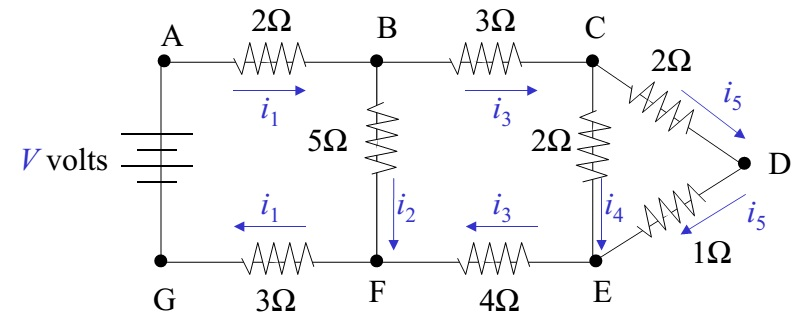
\includegraphics{circuit.png}}
\caption{Figure 1: Schéma du circuit électrique.}\end{figure}
\begin{enumerate}
\setcounter{enumi}{1}
\item {} 
Ecrire ces équations sous la forme de \(Ax=b\).

\end{enumerate}

voici les équations, si on applique les deux lois de \textbf{Kirchoff}.

Neoud \(B\).
\begin{gather}
\begin{split}i_1-i_2-i_3=0\end{split}\notag
\end{gather}
Noeud \(C\).
\begin{gather}
\begin{split}i_3-i_4-i_5=0\end{split}\notag
\end{gather}
Circuit fermé \(C_1\):
\begin{gather}
\begin{split}V-i_1(5\Omega)-i_2(5\Omega)=0\end{split}\notag
\end{gather}
Circuit fermé \(C_2\):
\begin{gather}
\begin{split}-i_3(7\Omega)-i_4(2\Omega)+i_2(5\Omega)=0\end{split}\notag
\end{gather}
Circuit fermé \(C_3\):
\begin{gather}
\begin{split}-i_5(3\Omega)+i_4(2\Omega)=0\end{split}\notag
\end{gather}
et donc le système est donné par:
\begin{gather}
\begin{split}\begin{pmatrix}
  1 & -1 & -1 & 0 &0 \\
  0 & 0  &  1 & -1 & -1\\
  5 & 5  & 0  & 0  & 0 \\
  0 & 5  & -7 & -2 & 0\\
  0 & 0 &0    & 2 & -3\\
\end{pmatrix}
\;\begin{pmatrix}
   i_1\\
   i_2\\
   i_3\\
   i_4\\
   i_5
\end{pmatrix}=\begin{pmatrix}
   0\\
   0\\
   V\\
   0\\
   0
\end{pmatrix}\end{split}\notag
\end{gather}

\bigskip\hrule{}\bigskip

\begin{enumerate}
\setcounter{enumi}{2}
\item {} 
Pour \(V=10\), résoudre le système \(Ax=b\) en utilisant l'opérateur \textbf{\textbackslash{}} de \emph{Matlab}.

\end{enumerate}

\textbf{Script principal}

\begin{Verbatim}[commandchars=\\\{\}]
\PYG{c}{\PYGZpc{}fixer la valeur de V}
\PYG{n}{V}\PYG{p}{=}\PYG{l+m+mi}{10}\PYG{p}{;}

\PYG{c}{\PYGZpc{}matrice A}
\PYG{n}{A}\PYG{p}{=}\PYG{p}{[}\PYG{l+m+mi}{1} \PYG{o}{\PYGZhy{}}\PYG{l+m+mi}{1} \PYG{o}{\PYGZhy{}}\PYG{l+m+mi}{1} \PYG{l+m+mi}{0} \PYG{l+m+mi}{0}\PYG{p}{;}
   \PYG{l+m+mi}{0}  \PYG{l+m+mi}{0} \PYG{l+m+mi}{1} \PYG{o}{\PYGZhy{}}\PYG{l+m+mi}{1} \PYG{l+m+mi}{0}\PYG{p}{;}
   \PYG{l+m+mi}{5}  \PYG{l+m+mi}{5} \PYG{l+m+mi}{0}  \PYG{l+m+mi}{0} \PYG{l+m+mi}{0}\PYG{p}{;}
   \PYG{l+m+mi}{0}  \PYG{l+m+mi}{5} \PYG{o}{\PYGZhy{}}\PYG{l+m+mi}{7} \PYG{o}{\PYGZhy{}}\PYG{l+m+mi}{2} \PYG{l+m+mi}{0}\PYG{p}{;}
   \PYG{l+m+mi}{0}  \PYG{l+m+mi}{0}  \PYG{l+m+mi}{0} \PYG{l+m+mi}{2} \PYG{o}{\PYGZhy{}}\PYG{l+m+mi}{3}\PYG{p}{]}\PYG{p}{;}

\PYG{c}{\PYGZpc{}vecteur b}
\PYG{n}{b}\PYG{p}{=}\PYG{p}{[}\PYG{n}{V}\PYG{p}{;}\PYG{l+m+mi}{0}\PYG{p}{;}\PYG{l+m+mi}{0}\PYG{p}{;}\PYG{l+m+mi}{0}\PYG{p}{;}\PYG{l+m+mi}{0}\PYG{p}{]}\PYG{p}{;}

\PYG{c}{\PYGZpc{}résolution par l\PYGZsq{}opérateur de matlab}
\PYG{n}{x}\PYG{p}{=}\PYG{n}{A}\PYG{o}{\PYGZbs{}}\PYG{n}{b}
\end{Verbatim}


\bigskip\hrule{}\bigskip

\begin{enumerate}
\setcounter{enumi}{3}
\item {} 
Ecrire une fonction qui résout un système \textbf{triangulaire inférieur}.

\end{enumerate}

\begin{Verbatim}[commandchars=\\\{\},numbers=left,firstnumber=1,stepnumber=1]
\PYG{k}{function}\PYG{+w}{ }x\PYG{p}{=}\PYG{n+nf}{rsl\PYGZus{}tri\PYGZus{}inf}\PYG{p}{(}A,b\PYG{p}{)}
\PYG{+w}{    }\PYG{c}{\PYGZpc{}\PYGZpc{} fonction pour résoudre un système inférieur Ax=b}
    
    \PYG{c}{\PYGZpc{}vérifier si le système est triangulaire}
    \PYG{n}{n}\PYG{p}{=}\PYG{n+nb}{length}\PYG{p}{(}\PYG{n}{A}\PYG{p}{)}\PYG{p}{;}
    
    \PYG{k}{for} \PYG{n+nb}{i}\PYG{p}{=}\PYG{l+m+mi}{1}\PYG{p}{:}\PYG{n}{n}
        \PYG{k}{for} \PYG{n+nb}{j}\PYG{p}{=}\PYG{n+nb}{i}\PYG{o}{+}\PYG{l+m+mi}{1}\PYG{p}{:}\PYG{n}{n}
            \PYG{k}{if}\PYG{p}{(}\PYG{n}{A}\PYG{p}{(}\PYG{n+nb}{i}\PYG{p}{,}\PYG{n+nb}{j}\PYG{p}{)}\PYG{o}{\PYGZti{}=}\PYG{l+m+mi}{0}\PYG{p}{)}
                \PYG{n}{error}\PYG{p}{(}\PYG{l+s}{\PYGZsq{}}\PYG{l+s}{matrice non trigulaire inf\PYGZsq{}}\PYG{p}{)}
            \PYG{k}{end}
        \PYG{k}{end}
    \PYG{k}{end}
    
    \PYG{c}{\PYGZpc{}vérifier si la matrice est régulière}
    \PYG{k}{for} \PYG{n+nb}{i}\PYG{p}{=}\PYG{l+m+mi}{1}\PYG{p}{:}\PYG{n}{n}
        \PYG{k}{if}\PYG{p}{(}\PYG{n}{A}\PYG{p}{(}\PYG{n+nb}{i}\PYG{p}{,}\PYG{n+nb}{i}\PYG{p}{)}\PYG{o}{==}\PYG{l+m+mi}{0}\PYG{p}{)}
            \PYG{n}{error}\PYG{p}{(}\PYG{l+s}{\PYGZsq{}}\PYG{l+s}{System singulier\PYGZsq{}}\PYG{p}{)}
        \PYG{k}{end}
    \PYG{k}{end}
    
    \PYG{c}{\PYGZpc{}résolution du system par l\PYGZsq{}algorithme de descente}
    
    \PYG{c}{\PYGZpc{}initialisation}
    \PYG{n}{x}\PYG{p}{=}\PYG{n+nb}{zeros}\PYG{p}{(}\PYG{n}{n}\PYG{p}{,}\PYG{l+m+mi}{1}\PYG{p}{)}\PYG{p}{;}
    \PYG{n}{x}\PYG{p}{(}\PYG{l+m+mi}{1}\PYG{p}{)}\PYG{p}{=}\PYG{n}{b}\PYG{p}{(}\PYG{l+m+mi}{1}\PYG{p}{)}\PYG{o}{/}\PYG{n}{A}\PYG{p}{(}\PYG{l+m+mi}{1}\PYG{p}{,}\PYG{l+m+mi}{1}\PYG{p}{)}\PYG{p}{;}
    
    \PYG{k}{for} \PYG{n+nb}{i}\PYG{p}{=}\PYG{l+m+mi}{2}\PYG{p}{:}\PYG{n}{n}
        \PYG{n}{x}\PYG{p}{(}\PYG{n+nb}{i}\PYG{p}{)}\PYG{p}{=}\PYG{p}{(}\PYG{n}{b}\PYG{p}{(}\PYG{n+nb}{i}\PYG{p}{)}\PYG{o}{\PYGZhy{}}\PYG{n}{A}\PYG{p}{(}\PYG{n+nb}{i}\PYG{p}{,}\PYG{l+m+mi}{1}\PYG{p}{:}\PYG{n+nb}{i}\PYG{o}{\PYGZhy{}}\PYG{l+m+mi}{1}\PYG{p}{)}\PYG{o}{*}\PYG{n}{x}\PYG{p}{(}\PYG{l+m+mi}{1}\PYG{p}{:}\PYG{n+nb}{i}\PYG{o}{\PYGZhy{}}\PYG{l+m+mi}{1}\PYG{p}{)}\PYG{p}{)}\PYG{o}{/}\PYG{n}{A}\PYG{p}{(}\PYG{n+nb}{i}\PYG{p}{,}\PYG{n+nb}{i}\PYG{p}{)}\PYG{p}{;}
    \PYG{k}{end}
    
\PYG{k}{end}
\end{Verbatim}

\begin{notice}{note}{Note:}
Dans la ligne (29) , la somme \(\sum_{j=1}^{i-1} A_{ij}\;x_j\) est formulée comme un \textbf{produit scalaire}.
\end{notice}


\bigskip\hrule{}\bigskip

\begin{enumerate}
\setcounter{enumi}{4}
\item {} 
Ecrire une fonction qui résout un système linéaire \textbf{triangulaire supérieur}

\end{enumerate}

\begin{Verbatim}[commandchars=\\\{\},numbers=left,firstnumber=1,stepnumber=1]
\PYG{k}{function}\PYG{+w}{ }x\PYG{p}{=}\PYG{n+nf}{rsl\PYGZus{}tri\PYGZus{}sup}\PYG{p}{(}A,b\PYG{p}{)}
\PYG{+w}{    }\PYG{c}{\PYGZpc{}\PYGZpc{} fonction pour résoudre un système supérieur Ax=b}
    
    \PYG{c}{\PYGZpc{}vérifier si le système est triangulaire}
    \PYG{n}{n}\PYG{p}{=}\PYG{n+nb}{length}\PYG{p}{(}\PYG{n}{A}\PYG{p}{)}\PYG{p}{;}
    
    \PYG{k}{for} \PYG{n+nb}{i}\PYG{p}{=}\PYG{l+m+mi}{1}\PYG{p}{:}\PYG{n}{n}
        \PYG{k}{for} \PYG{n+nb}{j}\PYG{p}{=}\PYG{l+m+mi}{1}\PYG{p}{:}\PYG{n+nb}{i}\PYG{o}{\PYGZhy{}}\PYG{l+m+mi}{1}
            \PYG{k}{if}\PYG{p}{(}\PYG{n}{A}\PYG{p}{(}\PYG{n+nb}{i}\PYG{p}{,}\PYG{n+nb}{j}\PYG{p}{)}\PYG{o}{\PYGZti{}=}\PYG{l+m+mi}{0}\PYG{p}{)}
                \PYG{n}{error}\PYG{p}{(}\PYG{l+s}{\PYGZsq{}}\PYG{l+s}{matrice non trigulaire inf\PYGZsq{}}\PYG{p}{)}
            \PYG{k}{end}
        \PYG{k}{end}
    \PYG{k}{end}
    
    \PYG{c}{\PYGZpc{}vérifier si la matrice est régulière}
    \PYG{k}{for} \PYG{n+nb}{i}\PYG{p}{=}\PYG{l+m+mi}{1}\PYG{p}{:}\PYG{n}{n}
        \PYG{k}{if}\PYG{p}{(}\PYG{n}{A}\PYG{p}{(}\PYG{n+nb}{i}\PYG{p}{,}\PYG{n+nb}{i}\PYG{p}{)}\PYG{o}{==}\PYG{l+m+mi}{0}\PYG{p}{)}
            \PYG{n}{error}\PYG{p}{(}\PYG{l+s}{\PYGZsq{}}\PYG{l+s}{System singulier\PYGZsq{}}\PYG{p}{)}
        \PYG{k}{end}
    \PYG{k}{end}
    
    \PYG{c}{\PYGZpc{}résolution du system par l\PYGZsq{}algorithme de montée}
    
    \PYG{c}{\PYGZpc{}initialisation}
    \PYG{n}{x}\PYG{p}{=}\PYG{n+nb}{zeros}\PYG{p}{(}\PYG{n}{n}\PYG{p}{,}\PYG{l+m+mi}{1}\PYG{p}{)}\PYG{p}{;}
    \PYG{n}{x}\PYG{p}{(}\PYG{n}{n}\PYG{p}{)}\PYG{p}{=}\PYG{n}{b}\PYG{p}{(}\PYG{n}{n}\PYG{p}{)}\PYG{o}{/}\PYG{n}{A}\PYG{p}{(}\PYG{n}{n}\PYG{p}{,}\PYG{n}{n}\PYG{p}{)}\PYG{p}{;}
    
    \PYG{c}{\PYGZpc{}boucle inversée}
    \PYG{k}{for} \PYG{n+nb}{i}\PYG{p}{=}\PYG{n}{n}\PYG{o}{\PYGZhy{}}\PYG{l+m+mi}{1}\PYG{p}{:}\PYG{o}{\PYGZhy{}}\PYG{l+m+mi}{1}\PYG{p}{:}\PYG{l+m+mi}{1}
        \PYG{n}{x}\PYG{p}{(}\PYG{n+nb}{i}\PYG{p}{)}\PYG{p}{=}\PYG{p}{(}\PYG{n}{b}\PYG{p}{(}\PYG{n+nb}{i}\PYG{p}{)}\PYG{o}{\PYGZhy{}}\PYG{n}{A}\PYG{p}{(}\PYG{n+nb}{i}\PYG{p}{,}\PYG{n+nb}{i}\PYG{o}{+}\PYG{l+m+mi}{1}\PYG{p}{:}\PYG{n}{n}\PYG{p}{)}\PYG{o}{*}\PYG{n}{x}\PYG{p}{(}\PYG{n+nb}{i}\PYG{o}{+}\PYG{l+m+mi}{1}\PYG{p}{:}\PYG{n}{n}\PYG{p}{)}\PYG{p}{)}\PYG{o}{/}\PYG{n}{A}\PYG{p}{(}\PYG{n+nb}{i}\PYG{p}{,}\PYG{n+nb}{i}\PYG{p}{)}\PYG{p}{;}
    \PYG{k}{end}
    
\PYG{k}{end}
\end{Verbatim}


\bigskip\hrule{}\bigskip

\begin{enumerate}
\setcounter{enumi}{5}
\item {} 
Ecrire une fonction qui résout un système linéaire \(Ax=b\) par la méthode de \textbf{LU}.

\end{enumerate}

\textbf{Algorithme LU}:

\begin{Verbatim}[commandchars=\\\{\}]
for k=1:n
  u(k,k)=a(k,k)

  for i=k+1:n
    l(i,k)=a(i,k)/u(k,k)
    u(k,i)=a(k,i)

  for i=k+1 : n
    for j=k+1:n
      a(i,j)=a(i,j)\PYGZhy{}l(i,k)u(k,j)
\end{Verbatim}

\begin{center}fonction decomposition
\end{center}
\begin{Verbatim}[commandchars=\\\{\},numbers=left,firstnumber=1,stepnumber=1]
\PYG{k}{function}\PYG{+w}{ }[L,U]\PYG{p}{=}\PYG{n+nf}{lu\PYGZus{}dcm}\PYG{p}{(}A\PYG{p}{)}
\PYG{c}{\PYGZpc{}\PYGZpc{} fonction pour obtenir la decomposition A=LU}
\PYG{c}{\PYGZpc{} les matrices L,U seront stockés dans A}

    \PYG{c}{\PYGZpc{}calculer la taille de A}
    \PYG{n}{n}\PYG{p}{=}\PYG{n+nb}{length}\PYG{p}{(}\PYG{n}{A}\PYG{p}{)}\PYG{p}{;}
    
    \PYG{c}{\PYGZpc{}Inialisation des deux matrices}
    \PYG{n}{L}\PYG{p}{=}\PYG{n+nb}{eye}\PYG{p}{(}\PYG{n}{n}\PYG{p}{)}\PYG{p}{;}
    \PYG{n}{U}\PYG{p}{=}\PYG{n+nb}{zeros}\PYG{p}{(}\PYG{n}{n}\PYG{p}{)}\PYG{p}{;}
    
    \PYG{k}{for} \PYG{n}{k}\PYG{p}{=}\PYG{l+m+mi}{1}\PYG{p}{:}\PYG{n}{n}
        
        \PYG{n}{U}\PYG{p}{(}\PYG{n}{k}\PYG{p}{,}\PYG{n}{k}\PYG{p}{)}\PYG{p}{=}\PYG{n}{A}\PYG{p}{(}\PYG{n}{k}\PYG{p}{,}\PYG{n}{k}\PYG{p}{)}\PYG{p}{;}
        
        \PYG{c}{\PYGZpc{}calcul de kieme ligne de U et kieme colonne de L}
        \PYG{k}{for} \PYG{n+nb}{i}\PYG{p}{=}\PYG{n}{k}\PYG{o}{+}\PYG{l+m+mi}{1}\PYG{p}{:}\PYG{n}{n}
            \PYG{n}{L}\PYG{p}{(}\PYG{n+nb}{i}\PYG{p}{,}\PYG{n}{k}\PYG{p}{)}\PYG{p}{=}\PYG{n}{A}\PYG{p}{(}\PYG{n+nb}{i}\PYG{p}{,}\PYG{n}{k}\PYG{p}{)}\PYG{o}{/}\PYG{n}{U}\PYG{p}{(}\PYG{n}{k}\PYG{p}{,}\PYG{n}{k}\PYG{p}{)}\PYG{p}{;}
            \PYG{n}{U}\PYG{p}{(}\PYG{n}{k}\PYG{p}{,}\PYG{n+nb}{i}\PYG{p}{)}\PYG{p}{=}\PYG{n}{A}\PYG{p}{(}\PYG{n}{k}\PYG{p}{,}\PYG{n+nb}{i}\PYG{p}{)}\PYG{p}{;}
        \PYG{k}{end}
        
        \PYG{c}{\PYGZpc{}transformation de la matrice intérieure }
        \PYG{k}{for} \PYG{n+nb}{i}\PYG{p}{=}\PYG{n}{k}\PYG{o}{+}\PYG{l+m+mi}{1}\PYG{p}{:}\PYG{n}{n}
            \PYG{k}{for} \PYG{n+nb}{j}\PYG{p}{=}\PYG{n}{k}\PYG{o}{+}\PYG{l+m+mi}{1}\PYG{p}{:}\PYG{n}{n}
                \PYG{n}{A}\PYG{p}{(}\PYG{n+nb}{i}\PYG{p}{,}\PYG{n+nb}{j}\PYG{p}{)}\PYG{p}{=}\PYG{n}{A}\PYG{p}{(}\PYG{n+nb}{i}\PYG{p}{,}\PYG{n+nb}{j}\PYG{p}{)}\PYG{o}{\PYGZhy{}}\PYG{n}{L}\PYG{p}{(}\PYG{n+nb}{i}\PYG{p}{,}\PYG{n}{k}\PYG{p}{)}\PYG{o}{*}\PYG{n}{U}\PYG{p}{(}\PYG{n}{k}\PYG{p}{,}\PYG{n+nb}{j}\PYG{p}{)}\PYG{p}{;}
            \PYG{k}{end}
        \PYG{k}{end}
    \PYG{k}{end}
\PYG{k}{end}
\end{Verbatim}

\begin{Verbatim}[commandchars=\\\{\},numbers=left,firstnumber=1,stepnumber=1]
\PYG{k}{function}\PYG{+w}{ }x\PYG{p}{=}\PYG{n+nf}{solve\PYGZus{}lu}\PYG{p}{(}A,b\PYG{p}{)}
\PYG{c}{\PYGZpc{}\PYGZpc{} fonction pour résoudre le système Ax=b avec la méthode LU}
\PYG{c}{\PYGZpc{} avec LU resultatn en deux matrices}


\PYG{c}{\PYGZpc{}decomposition LU}
\PYG{p}{[}\PYG{n}{L}\PYG{p}{,}\PYG{n}{U}\PYG{p}{]}\PYG{p}{=}\PYG{n}{lu\PYGZus{}dcm}\PYG{p}{(}\PYG{n}{A}\PYG{p}{)}\PYG{p}{;}

\PYG{c}{\PYGZpc{}resolution du système inférieur}
\PYG{n}{y1}\PYG{p}{=}\PYG{n}{rsl\PYGZus{}tri\PYGZus{}inf}\PYG{p}{(}\PYG{n}{L}\PYG{p}{,}\PYG{n}{b}\PYG{p}{)}\PYG{p}{;}

\PYG{c}{\PYGZpc{}resolution du système supérieur}
\PYG{n}{x}\PYG{p}{=}\PYG{n}{rsl\PYGZus{}tri\PYGZus{}sup}\PYG{p}{(}\PYG{n}{U}\PYG{p}{,}\PYG{n}{y1}\PYG{p}{)}\PYG{p}{;}
\PYG{k}{end}
\end{Verbatim}

\begin{center}script principal (suite)
\end{center}
\begin{Verbatim}[commandchars=\\\{\}]
\PYG{c}{\PYGZpc{}test de la solution avec lu\PYGZus{}dcm}
\PYG{n}{fprintf}\PYG{p}{(}\PYG{l+s}{\PYGZsq{}}\PYG{l+s}{solution par la decomposition LU:\PYGZsq{}}\PYG{p}{)}
\PYG{n}{x1}\PYG{p}{=}\PYG{n}{solve\PYGZus{}lu}\PYG{p}{(}\PYG{n}{A}\PYG{p}{,}\PYG{n}{b}\PYG{p}{)}
\end{Verbatim}


\bigskip\hrule{}\bigskip


\begin{notice}{note}{Note:}
On peut optimiser la mémoire du programme, en sauvegardant \(L\) et \(U\), dans  la même matrice.
\end{notice}

\textbf{Algorithme LU( 2)}:

\begin{Verbatim}[commandchars=\\\{\}]
for k=1:n\PYGZhy{}1
  for i=k+1:n
    a(i,k)=a(i,k)/a(k,k)

    for j=k+1:n
      a(i,j)=a(i,j)\PYGZhy{}l(i,k)*a(k,j)
\end{Verbatim}

A la fin du programme, la partie triangulaire sup de \(A\) est \(U\), et \(L\) est sauvegadée dans la partie inférieure \textbf{sans sa diagonale} (implicitement =1)

\begin{center}fonction decomposition compacte
\end{center}
\begin{Verbatim}[commandchars=\\\{\},numbers=left,firstnumber=1,stepnumber=1]
\PYG{k}{function}\PYG{+w}{ }LU\PYG{p}{=}\PYG{n+nf}{lu\PYGZus{}dcm2}\PYG{p}{(}A\PYG{p}{)}
\PYG{+w}{    }\PYG{c}{\PYGZpc{} fonction 2 pour calculer la décomposition LU de A}
    
    \PYG{c}{\PYGZpc{}nombre de ligne de A}
    \PYG{n}{n}\PYG{p}{=}\PYG{n+nb}{size}\PYG{p}{(}\PYG{n}{A}\PYG{p}{,}\PYG{l+m+mi}{1}\PYG{p}{)}\PYG{p}{;}
    \PYG{k}{for} \PYG{n}{k}\PYG{p}{=}\PYG{l+m+mi}{1}\PYG{p}{:}\PYG{n}{n}\PYG{o}{\PYGZhy{}}\PYG{l+m+mi}{1}
         \PYG{c}{\PYGZpc{}calcul du terme de la diagonale de U}
        \PYG{k}{for} \PYG{n+nb}{i}\PYG{p}{=}\PYG{n}{k}\PYG{o}{+}\PYG{l+m+mi}{1}\PYG{p}{:}\PYG{n}{n}
            \PYG{n}{A}\PYG{p}{(}\PYG{n+nb}{i}\PYG{p}{,}\PYG{n}{k}\PYG{p}{)}\PYG{p}{=}\PYG{n}{A}\PYG{p}{(}\PYG{n+nb}{i}\PYG{p}{,}\PYG{n}{k}\PYG{p}{)}\PYG{o}{/}\PYG{n}{A}\PYG{p}{(}\PYG{n}{k}\PYG{p}{,}\PYG{n}{k}\PYG{p}{)}\PYG{p}{;}
        
            
            \PYG{k}{for} \PYG{n+nb}{j}\PYG{p}{=}\PYG{n}{k}\PYG{o}{+}\PYG{l+m+mi}{1}\PYG{p}{:}\PYG{n}{n}
                \PYG{n}{A}\PYG{p}{(}\PYG{n+nb}{i}\PYG{p}{,}\PYG{n+nb}{j}\PYG{p}{)}\PYG{p}{=}\PYG{n}{A}\PYG{p}{(}\PYG{n+nb}{i}\PYG{p}{,}\PYG{n+nb}{j}\PYG{p}{)}\PYG{o}{\PYGZhy{}}\PYG{n}{A}\PYG{p}{(}\PYG{n+nb}{i}\PYG{p}{,}\PYG{n}{k}\PYG{p}{)}\PYG{o}{*}\PYG{n}{A}\PYG{p}{(}\PYG{n}{k}\PYG{p}{,}\PYG{n+nb}{j}\PYG{p}{)}\PYG{p}{;}
            \PYG{k}{end}
        \PYG{k}{end}
    \PYG{k}{end}
    \PYG{n}{LU}\PYG{p}{=}\PYG{n}{A}\PYG{p}{;}
\PYG{k}{end}
\end{Verbatim}

\begin{center}Résolution avec la matrice compacte
\end{center}
\begin{Verbatim}[commandchars=\\\{\},numbers=left,firstnumber=1,stepnumber=1]
\PYG{k}{function}\PYG{+w}{ }x\PYG{p}{=}\PYG{n+nf}{solve2\PYGZus{}lu}\PYG{p}{(}A,b\PYG{p}{)}
\PYG{c}{\PYGZpc{}\PYGZpc{} fonction pour résoudre le système Ax=b avec la méthode LU}
\PYG{c}{\PYGZpc{} avec LU stockée dans une seule matrice}


\PYG{c}{\PYGZpc{}decomposition LU}
\PYG{n}{LU}\PYG{p}{=}\PYG{n}{lu\PYGZus{}dcm2}\PYG{p}{(}\PYG{n}{A}\PYG{p}{)}\PYG{p}{;}

\PYG{c}{\PYGZpc{}extraire les matrices (L,U)( ce qui est contradictoire car le but était}
\PYG{c}{\PYGZpc{} de minimiser l\PYGZsq{}espace de stockage, donc avec cette stratégie il vaut}
\PYG{c}{\PYGZpc{}mieux adapter les méthode descente et montee pour ce type de matrice}

\PYG{n}{U}\PYG{p}{=}\PYG{n+nb}{triu}\PYG{p}{(}\PYG{n}{LU}\PYG{p}{)}\PYG{p}{;}
\PYG{n}{L}\PYG{p}{=}\PYG{n+nb}{tril}\PYG{p}{(}\PYG{n}{LU}\PYG{p}{)}\PYG{p}{;}
\PYG{c}{\PYGZpc{}introduire 1 dans la diagonale de L}
\PYG{n}{n}\PYG{p}{=}\PYG{n+nb}{size}\PYG{p}{(}\PYG{n}{L}\PYG{p}{,}\PYG{l+m+mi}{1}\PYG{p}{)}\PYG{p}{;}

\PYG{k}{for} \PYG{n+nb}{i}\PYG{p}{=}\PYG{l+m+mi}{1}\PYG{p}{:}\PYG{n}{n}
    \PYG{n}{L}\PYG{p}{(}\PYG{n+nb}{i}\PYG{p}{,}\PYG{n+nb}{i}\PYG{p}{)}\PYG{p}{=}\PYG{l+m+mi}{1}\PYG{p}{;}
\PYG{k}{end}

\PYG{c}{\PYGZpc{}resolution du système inférieur}
\PYG{n}{y1}\PYG{p}{=}\PYG{n}{rsl\PYGZus{}tri\PYGZus{}inf}\PYG{p}{(}\PYG{n}{L}\PYG{p}{,}\PYG{n}{b}\PYG{p}{)}\PYG{p}{;}

\PYG{c}{\PYGZpc{}resolution du système supérieur}
\PYG{n}{x}\PYG{p}{=}\PYG{n}{rsl\PYGZus{}tri\PYGZus{}sup}\PYG{p}{(}\PYG{n}{U}\PYG{p}{,}\PYG{n}{y1}\PYG{p}{)}\PYG{p}{;}

\PYG{k}{end}
\end{Verbatim}


\chapter{Tutorial on matrices}
\label{matrices:tutorial-on-matrices}\label{matrices::doc}

\section{Creating matrices}
\label{matrices:creating-matrices}
\begin{Verbatim}[commandchars=\\\{\}]
\PYG{c}{\PYGZsh{}importin sympy}
\PYG{k+kn}{from} \PYG{n+nn}{sympy} \PYG{k+kn}{import} \PYG{o}{*}
\PYG{n}{init\PYGZus{}printing}\PYG{p}{(}\PYG{n}{use\PYGZus{}latex}\PYG{o}{=}\PYG{n+nb+bp}{True}\PYG{p}{)}
\end{Verbatim}

\begin{Verbatim}[commandchars=\\\{\}]
\PYG{n}{M}\PYG{o}{=}\PYG{n}{Matrix}\PYG{p}{(}\PYG{p}{[}\PYG{p}{[}\PYG{l+m+mi}{1}\PYG{p}{,}\PYG{l+m+mi}{2}\PYG{p}{]}\PYG{p}{,}\PYG{p}{[}\PYG{l+m+mi}{3}\PYG{p}{,}\PYG{l+m+mi}{4}\PYG{p}{]}\PYG{p}{,}\PYG{p}{[}\PYG{l+m+mi}{4}\PYG{p}{,}\PYG{l+m+mi}{5}\PYG{p}{]}\PYG{p}{]}\PYG{p}{)}
\end{Verbatim}


\section{définition de la matrice}
\label{matrices:definition-de-la-matrice}
\begin{Verbatim}[commandchars=\\\{\}]
\PYG{c}{\PYGZsh{}définir la matrice en lambda}
\PYG{n}{lamda}\PYG{o}{=}\PYG{n}{Symbol}\PYG{p}{(}\PYG{l+s}{\PYGZsq{}}\PYG{l+s}{lamda}\PYG{l+s}{\PYGZsq{}}\PYG{p}{)}
\end{Verbatim}

\begin{Verbatim}[commandchars=\\\{\}]
\PYG{n}{lamda}
\end{Verbatim}
\begin{gather}
\begin{split}\lambda\end{split}\notag
\end{gather}
Maintenant on va définir la fonction pour calculer \(M_{ij}\).

\begin{Verbatim}[commandchars=\\\{\}]
\PYG{k}{def} \PYG{n+nf}{f}\PYG{p}{(}\PYG{n}{i}\PYG{p}{,}\PYG{n}{j}\PYG{p}{)}\PYG{p}{:}
    \PYG{c}{\PYGZsh{}element de la diagonale}
    \PYG{k}{if}\PYG{p}{(}\PYG{n}{i}\PYG{o}{==}\PYG{n}{j}\PYG{p}{)}\PYG{p}{:}
        \PYG{k}{return} \PYG{l+m+mi}{1}\PYG{o}{+}\PYG{l+m+mi}{2}\PYG{o}{*}\PYG{n}{lamda}\PYG{o}{*}\PYG{o}{*}\PYG{l+m+mi}{2}
    \PYG{k}{elif}\PYG{p}{(}\PYG{n}{i}\PYG{o}{==}\PYG{n}{j}\PYG{o}{+}\PYG{l+m+mi}{1} \PYG{o+ow}{or} \PYG{n}{i}\PYG{o}{==}\PYG{n}{j}\PYG{o}{\PYGZhy{}}\PYG{l+m+mi}{1}\PYG{p}{)}\PYG{p}{:}
        \PYG{k}{return} \PYG{o}{\PYGZhy{}}\PYG{n}{lamda}\PYG{o}{*}\PYG{o}{*}\PYG{l+m+mi}{2}\PYG{p}{;}
    \PYG{k}{else}\PYG{p}{:}
        \PYG{k}{return} \PYG{l+m+mi}{0}
\end{Verbatim}

construire une matrice de taille \(5\), en utilisant la fonction
\(f\).

\begin{Verbatim}[commandchars=\\\{\}]
\PYG{n}{M}\PYG{o}{=}\PYG{n}{Matrix}\PYG{p}{(}\PYG{l+m+mi}{3}\PYG{p}{,}\PYG{l+m+mi}{3}\PYG{p}{,}\PYG{n}{f}\PYG{p}{)}\PYG{p}{;}
\end{Verbatim}

Correction de la première et dérnière ligne

\begin{Verbatim}[commandchars=\\\{\}]
\PYG{n}{M}\PYG{p}{[}\PYG{l+m+mi}{0}\PYG{p}{,}\PYG{l+m+mi}{0}\PYG{p}{]}\PYG{o}{=}\PYG{l+m+mi}{1}\PYG{o}{+}\PYG{n}{lamda}\PYG{o}{*}\PYG{o}{*}\PYG{l+m+mi}{2}\PYG{p}{;} \PYG{n}{M}\PYG{p}{[}\PYG{o}{\PYGZhy{}}\PYG{l+m+mi}{1}\PYG{p}{,}\PYG{o}{\PYGZhy{}}\PYG{l+m+mi}{1}\PYG{p}{]}\PYG{o}{=}\PYG{l+m+mi}{1}\PYG{o}{+}\PYG{n}{lamda}\PYG{o}{*}\PYG{o}{*}\PYG{l+m+mi}{2}
\end{Verbatim}

\begin{Verbatim}[commandchars=\\\{\}]
\PYG{n}{M}
\end{Verbatim}
\begin{gather}
\begin{split}\left[\begin{matrix}\lambda^{2} + 1 & - \lambda^{2} & 0\\- \lambda^{2} & 2 \lambda^{2} + 1 & - \lambda^{2}\\0 & - \lambda^{2} & \lambda^{2} + 1\end{matrix}\right]\end{split}\notag
\end{gather}
maintenant on va inverser la matrice

\begin{Verbatim}[commandchars=\\\{\}]
\PYG{n}{L}\PYG{o}{=}\PYG{n}{M}\PYG{o}{.}\PYG{n}{inv}\PYG{p}{(}\PYG{p}{)}
\end{Verbatim}

\begin{Verbatim}[commandchars=\\\{\}]
\PYG{n}{L}
\end{Verbatim}
\begin{gather}
\begin{split}\left[\begin{matrix}\frac{\lambda^{8}}{\left(\lambda^{4} + 3 \lambda^{2} + 1\right) \left(3 \lambda^{4} + 4 \lambda^{2} + 1\right)} + \frac{\lambda^{4}}{\left(\lambda^{2} + 1\right) \left(\lambda^{4} + 3 \lambda^{2} + 1\right)} + \frac{1}{\lambda^{2} + 1} & \frac{\lambda^{6} \left(\lambda^{2} + 1\right)}{\left(\lambda^{4} + 3 \lambda^{2} + 1\right) \left(3 \lambda^{4} + 4 \lambda^{2} + 1\right)} + \frac{\lambda^{2}}{\lambda^{4} + 3 \lambda^{2} + 1} & \frac{\lambda^{4}}{3 \lambda^{4} + 4 \lambda^{2} + 1}\\\frac{\lambda^{6} \left(\lambda^{2} + 1\right)}{\left(\lambda^{4} + 3 \lambda^{2} + 1\right) \left(3 \lambda^{4} + 4 \lambda^{2} + 1\right)} + \frac{\lambda^{2}}{\lambda^{4} + 3 \lambda^{2} + 1} & \frac{\lambda^{4} \left(\lambda^{2} + 1\right)^{2}}{\left(\lambda^{4} + 3 \lambda^{2} + 1\right) \left(3 \lambda^{4} + 4 \lambda^{2} + 1\right)} + \frac{\lambda^{2} + 1}{\lambda^{4} + 3 \lambda^{2} + 1} & \frac{\lambda^{2} \left(\lambda^{2} + 1\right)}{3 \lambda^{4} + 4 \lambda^{2} + 1}\\\frac{\lambda^{4}}{3 \lambda^{4} + 4 \lambda^{2} + 1} & \frac{\lambda^{2} \left(\lambda^{2} + 1\right)}{3 \lambda^{4} + 4 \lambda^{2} + 1} & \frac{\lambda^{4} + 3 \lambda^{2} + 1}{3 \lambda^{4} + 4 \lambda^{2} + 1}\end{matrix}\right]\end{split}\notag
\end{gather}
\begin{Verbatim}[commandchars=\\\{\}]
\PYG{n}{L}\PYG{o}{.}\PYG{n}{simplify}\PYG{p}{(}\PYG{p}{)}
\end{Verbatim}

\begin{Verbatim}[commandchars=\\\{\}]
\PYG{n}{L}
\end{Verbatim}
\begin{gather}
\begin{split}\left[\begin{matrix}\frac{\lambda^{4} + 3 \lambda^{2} + 1}{3 \lambda^{4} + 4 \lambda^{2} + 1} & \frac{\lambda^{2}}{3 \lambda^{2} + 1} & \frac{\lambda^{4}}{3 \lambda^{4} + 4 \lambda^{2} + 1}\\\frac{\lambda^{2}}{3 \lambda^{2} + 1} & \frac{\lambda^{2} + 1}{3 \lambda^{2} + 1} & \frac{\lambda^{2}}{3 \lambda^{2} + 1}\\\frac{\lambda^{4}}{3 \lambda^{4} + 4 \lambda^{2} + 1} & \frac{\lambda^{2}}{3 \lambda^{2} + 1} & \frac{\lambda^{4} + 3 \lambda^{2} + 1}{3 \lambda^{4} + 4 \lambda^{2} + 1}\end{matrix}\right]\end{split}\notag
\end{gather}
\begin{Verbatim}[commandchars=\\\{\}]
\PYG{n}{S}\PYG{o}{=}\PYG{n}{Matrix}\PYG{p}{(}\PYG{l+m+mi}{5}\PYG{p}{,}\PYG{l+m+mi}{5}\PYG{p}{,}\PYG{n}{f}\PYG{p}{)}
\end{Verbatim}

\begin{Verbatim}[commandchars=\\\{\}]
\PYG{n}{S}\PYG{p}{[}\PYG{l+m+mi}{0}\PYG{p}{,}\PYG{l+m+mi}{0}\PYG{p}{]}\PYG{o}{=}\PYG{l+m+mi}{1}\PYG{o}{+}\PYG{n}{lamda}\PYG{o}{*}\PYG{o}{*}\PYG{l+m+mi}{2}\PYG{p}{;} \PYG{n}{S}\PYG{p}{[}\PYG{o}{\PYGZhy{}}\PYG{l+m+mi}{1}\PYG{p}{,}\PYG{o}{\PYGZhy{}}\PYG{l+m+mi}{1}\PYG{p}{]}\PYG{o}{=}\PYG{l+m+mi}{1}\PYG{o}{+}\PYG{n}{lamda}\PYG{o}{*}\PYG{o}{*}\PYG{l+m+mi}{2}\PYG{p}{;}
\end{Verbatim}

\begin{Verbatim}[commandchars=\\\{\}]
\PYG{n}{S}
\end{Verbatim}
\begin{gather}
\begin{split}\left[\begin{matrix}\lambda^{2} + 1 & - \lambda^{2} & 0 & 0 & 0\\- \lambda^{2} & 2 \lambda^{2} + 1 & - \lambda^{2} & 0 & 0\\0 & - \lambda^{2} & 2 \lambda^{2} + 1 & - \lambda^{2} & 0\\0 & 0 & - \lambda^{2} & 2 \lambda^{2} + 1 & - \lambda^{2}\\0 & 0 & 0 & - \lambda^{2} & \lambda^{2} + 1\end{matrix}\right]\end{split}\notag
\end{gather}
\begin{Verbatim}[commandchars=\\\{\}]
\PYG{n}{L}\PYG{o}{=}\PYG{n}{S}\PYG{o}{.}\PYG{n}{inv}\PYG{p}{(}\PYG{p}{)}
\end{Verbatim}

\begin{Verbatim}[commandchars=\\\{\}]
\PYG{n}{L}
\end{Verbatim}
\begin{gather}
\begin{split}\left[\begin{matrix}\frac{\lambda^{16}}{\left(\lambda^{8} + 10 \lambda^{6} + 15 \lambda^{4} + 7 \lambda^{2} + 1\right) \left(5 \lambda^{8} + 20 \lambda^{6} + 21 \lambda^{4} + 8 \lambda^{2} + 1\right)} + \frac{\lambda^{12}}{\left(\lambda^{6} + 6 \lambda^{4} + 5 \lambda^{2} + 1\right) \left(\lambda^{8} + 10 \lambda^{6} + 15 \lambda^{4} + 7 \lambda^{2} + 1\right)} + \frac{\lambda^{8}}{\left(\lambda^{4} + 3 \lambda^{2} + 1\right) \left(\lambda^{6} + 6 \lambda^{4} + 5 \lambda^{2} + 1\right)} + \frac{\lambda^{4}}{\left(\lambda^{2} + 1\right) \left(\lambda^{4} + 3 \lambda^{2} + 1\right)} + \frac{1}{\lambda^{2} + 1} & \frac{\lambda^{14} \left(\lambda^{2} + 1\right)}{\left(\lambda^{8} + 10 \lambda^{6} + 15 \lambda^{4} + 7 \lambda^{2} + 1\right) \left(5 \lambda^{8} + 20 \lambda^{6} + 21 \lambda^{4} + 8 \lambda^{2} + 1\right)} + \frac{\lambda^{10} \left(\lambda^{2} + 1\right)}{\left(\lambda^{6} + 6 \lambda^{4} + 5 \lambda^{2} + 1\right) \left(\lambda^{8} + 10 \lambda^{6} + 15 \lambda^{4} + 7 \lambda^{2} + 1\right)} + \frac{\lambda^{6} \left(\lambda^{2} + 1\right)}{\left(\lambda^{4} + 3 \lambda^{2} + 1\right) \left(\lambda^{6} + 6 \lambda^{4} + 5 \lambda^{2} + 1\right)} + \frac{\lambda^{2}}{\lambda^{4} + 3 \lambda^{2} + 1} & \frac{\lambda^{12} \left(\lambda^{4} + 3 \lambda^{2} + 1\right)}{\left(\lambda^{8} + 10 \lambda^{6} + 15 \lambda^{4} + 7 \lambda^{2} + 1\right) \left(5 \lambda^{8} + 20 \lambda^{6} + 21 \lambda^{4} + 8 \lambda^{2} + 1\right)} + \frac{\lambda^{8} \left(\lambda^{4} + 3 \lambda^{2} + 1\right)}{\left(\lambda^{6} + 6 \lambda^{4} + 5 \lambda^{2} + 1\right) \left(\lambda^{8} + 10 \lambda^{6} + 15 \lambda^{4} + 7 \lambda^{2} + 1\right)} + \frac{\lambda^{4}}{\lambda^{6} + 6 \lambda^{4} + 5 \lambda^{2} + 1} & \frac{\lambda^{10} \left(\lambda^{6} + 6 \lambda^{4} + 5 \lambda^{2} + 1\right)}{\left(\lambda^{8} + 10 \lambda^{6} + 15 \lambda^{4} + 7 \lambda^{2} + 1\right) \left(5 \lambda^{8} + 20 \lambda^{6} + 21 \lambda^{4} + 8 \lambda^{2} + 1\right)} + \frac{\lambda^{6}}{\lambda^{8} + 10 \lambda^{6} + 15 \lambda^{4} + 7 \lambda^{2} + 1} & \frac{\lambda^{8}}{5 \lambda^{8} + 20 \lambda^{6} + 21 \lambda^{4} + 8 \lambda^{2} + 1}\\\frac{\lambda^{14} \left(\lambda^{2} + 1\right)}{\left(\lambda^{8} + 10 \lambda^{6} + 15 \lambda^{4} + 7 \lambda^{2} + 1\right) \left(5 \lambda^{8} + 20 \lambda^{6} + 21 \lambda^{4} + 8 \lambda^{2} + 1\right)} + \frac{\lambda^{10} \left(\lambda^{2} + 1\right)}{\left(\lambda^{6} + 6 \lambda^{4} + 5 \lambda^{2} + 1\right) \left(\lambda^{8} + 10 \lambda^{6} + 15 \lambda^{4} + 7 \lambda^{2} + 1\right)} + \frac{\lambda^{6} \left(\lambda^{2} + 1\right)}{\left(\lambda^{4} + 3 \lambda^{2} + 1\right) \left(\lambda^{6} + 6 \lambda^{4} + 5 \lambda^{2} + 1\right)} + \frac{\lambda^{2}}{\lambda^{4} + 3 \lambda^{2} + 1} & \frac{\lambda^{12} \left(\lambda^{2} + 1\right)^{2}}{\left(\lambda^{8} + 10 \lambda^{6} + 15 \lambda^{4} + 7 \lambda^{2} + 1\right) \left(5 \lambda^{8} + 20 \lambda^{6} + 21 \lambda^{4} + 8 \lambda^{2} + 1\right)} + \frac{\lambda^{8} \left(\lambda^{2} + 1\right)^{2}}{\left(\lambda^{6} + 6 \lambda^{4} + 5 \lambda^{2} + 1\right) \left(\lambda^{8} + 10 \lambda^{6} + 15 \lambda^{4} + 7 \lambda^{2} + 1\right)} + \frac{\lambda^{4} \left(\lambda^{2} + 1\right)^{2}}{\left(\lambda^{4} + 3 \lambda^{2} + 1\right) \left(\lambda^{6} + 6 \lambda^{4} + 5 \lambda^{2} + 1\right)} + \frac{\lambda^{2} + 1}{\lambda^{4} + 3 \lambda^{2} + 1} & \frac{\lambda^{10} \left(\lambda^{2} + 1\right) \left(\lambda^{4} + 3 \lambda^{2} + 1\right)}{\left(\lambda^{8} + 10 \lambda^{6} + 15 \lambda^{4} + 7 \lambda^{2} + 1\right) \left(5 \lambda^{8} + 20 \lambda^{6} + 21 \lambda^{4} + 8 \lambda^{2} + 1\right)} + \frac{\lambda^{6} \left(\lambda^{2} + 1\right) \left(\lambda^{4} + 3 \lambda^{2} + 1\right)}{\left(\lambda^{6} + 6 \lambda^{4} + 5 \lambda^{2} + 1\right) \left(\lambda^{8} + 10 \lambda^{6} + 15 \lambda^{4} + 7 \lambda^{2} + 1\right)} + \frac{\lambda^{2} \left(\lambda^{2} + 1\right)}{\lambda^{6} + 6 \lambda^{4} + 5 \lambda^{2} + 1} & \frac{\lambda^{8} \left(\lambda^{2} + 1\right) \left(\lambda^{6} + 6 \lambda^{4} + 5 \lambda^{2} + 1\right)}{\left(\lambda^{8} + 10 \lambda^{6} + 15 \lambda^{4} + 7 \lambda^{2} + 1\right) \left(5 \lambda^{8} + 20 \lambda^{6} + 21 \lambda^{4} + 8 \lambda^{2} + 1\right)} + \frac{\lambda^{4} \left(\lambda^{2} + 1\right)}{\lambda^{8} + 10 \lambda^{6} + 15 \lambda^{4} + 7 \lambda^{2} + 1} & \frac{\lambda^{6} \left(\lambda^{2} + 1\right)}{5 \lambda^{8} + 20 \lambda^{6} + 21 \lambda^{4} + 8 \lambda^{2} + 1}\\\frac{\lambda^{12} \left(\lambda^{4} + 3 \lambda^{2} + 1\right)}{\left(\lambda^{8} + 10 \lambda^{6} + 15 \lambda^{4} + 7 \lambda^{2} + 1\right) \left(5 \lambda^{8} + 20 \lambda^{6} + 21 \lambda^{4} + 8 \lambda^{2} + 1\right)} + \frac{\lambda^{8} \left(\lambda^{4} + 3 \lambda^{2} + 1\right)}{\left(\lambda^{6} + 6 \lambda^{4} + 5 \lambda^{2} + 1\right) \left(\lambda^{8} + 10 \lambda^{6} + 15 \lambda^{4} + 7 \lambda^{2} + 1\right)} + \frac{\lambda^{4}}{\lambda^{6} + 6 \lambda^{4} + 5 \lambda^{2} + 1} & \frac{\lambda^{10} \left(\lambda^{2} + 1\right) \left(\lambda^{4} + 3 \lambda^{2} + 1\right)}{\left(\lambda^{8} + 10 \lambda^{6} + 15 \lambda^{4} + 7 \lambda^{2} + 1\right) \left(5 \lambda^{8} + 20 \lambda^{6} + 21 \lambda^{4} + 8 \lambda^{2} + 1\right)} + \frac{\lambda^{6} \left(\lambda^{2} + 1\right) \left(\lambda^{4} + 3 \lambda^{2} + 1\right)}{\left(\lambda^{6} + 6 \lambda^{4} + 5 \lambda^{2} + 1\right) \left(\lambda^{8} + 10 \lambda^{6} + 15 \lambda^{4} + 7 \lambda^{2} + 1\right)} + \frac{\lambda^{2} \left(\lambda^{2} + 1\right)}{\lambda^{6} + 6 \lambda^{4} + 5 \lambda^{2} + 1} & \frac{\lambda^{8} \left(\lambda^{4} + 3 \lambda^{2} + 1\right)^{2}}{\left(\lambda^{8} + 10 \lambda^{6} + 15 \lambda^{4} + 7 \lambda^{2} + 1\right) \left(5 \lambda^{8} + 20 \lambda^{6} + 21 \lambda^{4} + 8 \lambda^{2} + 1\right)} + \frac{\lambda^{4} \left(\lambda^{4} + 3 \lambda^{2} + 1\right)^{2}}{\left(\lambda^{6} + 6 \lambda^{4} + 5 \lambda^{2} + 1\right) \left(\lambda^{8} + 10 \lambda^{6} + 15 \lambda^{4} + 7 \lambda^{2} + 1\right)} + \frac{\lambda^{4} + 3 \lambda^{2} + 1}{\lambda^{6} + 6 \lambda^{4} + 5 \lambda^{2} + 1} & \frac{\lambda^{6} \left(\lambda^{4} + 3 \lambda^{2} + 1\right) \left(\lambda^{6} + 6 \lambda^{4} + 5 \lambda^{2} + 1\right)}{\left(\lambda^{8} + 10 \lambda^{6} + 15 \lambda^{4} + 7 \lambda^{2} + 1\right) \left(5 \lambda^{8} + 20 \lambda^{6} + 21 \lambda^{4} + 8 \lambda^{2} + 1\right)} + \frac{\lambda^{2} \left(\lambda^{4} + 3 \lambda^{2} + 1\right)}{\lambda^{8} + 10 \lambda^{6} + 15 \lambda^{4} + 7 \lambda^{2} + 1} & \frac{\lambda^{4} \left(\lambda^{4} + 3 \lambda^{2} + 1\right)}{5 \lambda^{8} + 20 \lambda^{6} + 21 \lambda^{4} + 8 \lambda^{2} + 1}\\\frac{\lambda^{10} \left(\lambda^{6} + 6 \lambda^{4} + 5 \lambda^{2} + 1\right)}{\left(\lambda^{8} + 10 \lambda^{6} + 15 \lambda^{4} + 7 \lambda^{2} + 1\right) \left(5 \lambda^{8} + 20 \lambda^{6} + 21 \lambda^{4} + 8 \lambda^{2} + 1\right)} + \frac{\lambda^{6}}{\lambda^{8} + 10 \lambda^{6} + 15 \lambda^{4} + 7 \lambda^{2} + 1} & \frac{\lambda^{8} \left(\lambda^{2} + 1\right) \left(\lambda^{6} + 6 \lambda^{4} + 5 \lambda^{2} + 1\right)}{\left(\lambda^{8} + 10 \lambda^{6} + 15 \lambda^{4} + 7 \lambda^{2} + 1\right) \left(5 \lambda^{8} + 20 \lambda^{6} + 21 \lambda^{4} + 8 \lambda^{2} + 1\right)} + \frac{\lambda^{4} \left(\lambda^{2} + 1\right)}{\lambda^{8} + 10 \lambda^{6} + 15 \lambda^{4} + 7 \lambda^{2} + 1} & \frac{\lambda^{6} \left(\lambda^{4} + 3 \lambda^{2} + 1\right) \left(\lambda^{6} + 6 \lambda^{4} + 5 \lambda^{2} + 1\right)}{\left(\lambda^{8} + 10 \lambda^{6} + 15 \lambda^{4} + 7 \lambda^{2} + 1\right) \left(5 \lambda^{8} + 20 \lambda^{6} + 21 \lambda^{4} + 8 \lambda^{2} + 1\right)} + \frac{\lambda^{2} \left(\lambda^{4} + 3 \lambda^{2} + 1\right)}{\lambda^{8} + 10 \lambda^{6} + 15 \lambda^{4} + 7 \lambda^{2} + 1} & \frac{\lambda^{4} \left(\lambda^{6} + 6 \lambda^{4} + 5 \lambda^{2} + 1\right)^{2}}{\left(\lambda^{8} + 10 \lambda^{6} + 15 \lambda^{4} + 7 \lambda^{2} + 1\right) \left(5 \lambda^{8} + 20 \lambda^{6} + 21 \lambda^{4} + 8 \lambda^{2} + 1\right)} + \frac{\lambda^{6} + 6 \lambda^{4} + 5 \lambda^{2} + 1}{\lambda^{8} + 10 \lambda^{6} + 15 \lambda^{4} + 7 \lambda^{2} + 1} & \frac{\lambda^{2} \left(\lambda^{6} + 6 \lambda^{4} + 5 \lambda^{2} + 1\right)}{5 \lambda^{8} + 20 \lambda^{6} + 21 \lambda^{4} + 8 \lambda^{2} + 1}\\\frac{\lambda^{8}}{5 \lambda^{8} + 20 \lambda^{6} + 21 \lambda^{4} + 8 \lambda^{2} + 1} & \frac{\lambda^{6} \left(\lambda^{2} + 1\right)}{5 \lambda^{8} + 20 \lambda^{6} + 21 \lambda^{4} + 8 \lambda^{2} + 1} & \frac{\lambda^{4} \left(\lambda^{4} + 3 \lambda^{2} + 1\right)}{5 \lambda^{8} + 20 \lambda^{6} + 21 \lambda^{4} + 8 \lambda^{2} + 1} & \frac{\lambda^{2} \left(\lambda^{6} + 6 \lambda^{4} + 5 \lambda^{2} + 1\right)}{5 \lambda^{8} + 20 \lambda^{6} + 21 \lambda^{4} + 8 \lambda^{2} + 1} & \frac{\lambda^{8} + 10 \lambda^{6} + 15 \lambda^{4} + 7 \lambda^{2} + 1}{5 \lambda^{8} + 20 \lambda^{6} + 21 \lambda^{4} + 8 \lambda^{2} + 1}\end{matrix}\right]\end{split}\notag
\end{gather}
\begin{Verbatim}[commandchars=\\\{\}]
\PYG{n}{L}\PYG{o}{.}\PYG{n}{simplify}\PYG{p}{(}\PYG{p}{)}
\end{Verbatim}

\begin{Verbatim}[commandchars=\\\{\}]
\PYG{n}{L}
\end{Verbatim}
\begin{gather}
\begin{split}\left[\begin{matrix}\frac{\lambda^{8} + 10 \lambda^{6} + 15 \lambda^{4} + 7 \lambda^{2} + 1}{5 \lambda^{8} + 20 \lambda^{6} + 21 \lambda^{4} + 8 \lambda^{2} + 1} & \frac{\lambda^{2} \left(\lambda^{6} + 6 \lambda^{4} + 5 \lambda^{2} + 1\right)}{5 \lambda^{8} + 20 \lambda^{6} + 21 \lambda^{4} + 8 \lambda^{2} + 1} & \frac{\lambda^{4}}{5 \lambda^{4} + 5 \lambda^{2} + 1} & \frac{\lambda^{6} \left(\lambda^{2} + 1\right)}{5 \lambda^{8} + 20 \lambda^{6} + 21 \lambda^{4} + 8 \lambda^{2} + 1} & \frac{\lambda^{8}}{5 \lambda^{8} + 20 \lambda^{6} + 21 \lambda^{4} + 8 \lambda^{2} + 1}\\\frac{\lambda^{2} \left(\lambda^{6} + 6 \lambda^{4} + 5 \lambda^{2} + 1\right)}{5 \lambda^{8} + 20 \lambda^{6} + 21 \lambda^{4} + 8 \lambda^{2} + 1} & \frac{\lambda^{8} + 7 \lambda^{6} + 11 \lambda^{4} + 6 \lambda^{2} + 1}{5 \lambda^{8} + 20 \lambda^{6} + 21 \lambda^{4} + 8 \lambda^{2} + 1} & \frac{\lambda^{2} \left(\lambda^{2} + 1\right)}{5 \lambda^{4} + 5 \lambda^{2} + 1} & \frac{\lambda^{4} \left(\lambda^{4} + 2 \lambda^{2} + 1\right)}{5 \lambda^{8} + 20 \lambda^{6} + 21 \lambda^{4} + 8 \lambda^{2} + 1} & \frac{\lambda^{6} \left(\lambda^{2} + 1\right)}{5 \lambda^{8} + 20 \lambda^{6} + 21 \lambda^{4} + 8 \lambda^{2} + 1}\\\frac{\lambda^{4}}{5 \lambda^{4} + 5 \lambda^{2} + 1} & \frac{\lambda^{2} \left(\lambda^{2} + 1\right)}{5 \lambda^{4} + 5 \lambda^{2} + 1} & \frac{\lambda^{4} + 3 \lambda^{2} + 1}{5 \lambda^{4} + 5 \lambda^{2} + 1} & \frac{\lambda^{2} \left(\lambda^{2} + 1\right)}{5 \lambda^{4} + 5 \lambda^{2} + 1} & \frac{\lambda^{4}}{5 \lambda^{4} + 5 \lambda^{2} + 1}\\\frac{\lambda^{6} \left(\lambda^{2} + 1\right)}{5 \lambda^{8} + 20 \lambda^{6} + 21 \lambda^{4} + 8 \lambda^{2} + 1} & \frac{\lambda^{4} \left(\lambda^{4} + 2 \lambda^{2} + 1\right)}{5 \lambda^{8} + 20 \lambda^{6} + 21 \lambda^{4} + 8 \lambda^{2} + 1} & \frac{\lambda^{2} \left(\lambda^{2} + 1\right)}{5 \lambda^{4} + 5 \lambda^{2} + 1} & \frac{\lambda^{8} + 7 \lambda^{6} + 11 \lambda^{4} + 6 \lambda^{2} + 1}{5 \lambda^{8} + 20 \lambda^{6} + 21 \lambda^{4} + 8 \lambda^{2} + 1} & \frac{\lambda^{2} \left(\lambda^{6} + 6 \lambda^{4} + 5 \lambda^{2} + 1\right)}{5 \lambda^{8} + 20 \lambda^{6} + 21 \lambda^{4} + 8 \lambda^{2} + 1}\\\frac{\lambda^{8}}{5 \lambda^{8} + 20 \lambda^{6} + 21 \lambda^{4} + 8 \lambda^{2} + 1} & \frac{\lambda^{6} \left(\lambda^{2} + 1\right)}{5 \lambda^{8} + 20 \lambda^{6} + 21 \lambda^{4} + 8 \lambda^{2} + 1} & \frac{\lambda^{4}}{5 \lambda^{4} + 5 \lambda^{2} + 1} & \frac{\lambda^{2} \left(\lambda^{6} + 6 \lambda^{4} + 5 \lambda^{2} + 1\right)}{5 \lambda^{8} + 20 \lambda^{6} + 21 \lambda^{4} + 8 \lambda^{2} + 1} & \frac{\lambda^{8} + 10 \lambda^{6} + 15 \lambda^{4} + 7 \lambda^{2} + 1}{5 \lambda^{8} + 20 \lambda^{6} + 21 \lambda^{4} + 8 \lambda^{2} + 1}\end{matrix}\right]\end{split}\notag
\end{gather}

\chapter{Indices et Tables}
\label{index:indices-et-tables}\begin{itemize}
\item {} 
\emph{genindex}

\item {} 
\emph{modindex}

\item {} 
\emph{search}

\end{itemize}



\renewcommand{\indexname}{Index}
\printindex
\end{document}
